\chapter{Entity-Based Models}
\label{chapt:entity_based_models}
%
The coherence of a text is interpreted by means of relations, including both explicit and implicit, among sentences of a text. 
Various types of relations may exist between sentences. 
Entity-based relations are taken as a major relation type because entities are a prominent information for NLP applications (e.g., question answering) and information retrieval systems. 
So it is required to have a definition of an entity.
We refer to an entity as a person, an object or abstraction that exists (or could exist) external world to the text. 
Entities have been extracted as important information in Information Extraction (IE) applications. 
For instance, in entity disambiguation -- as a well-known task in IE -- the goal is to extract word spans that refer to either a person, organization, time, and etc. 
Pieces of a text that we use to refer to an entity are named mentions. 
Entity can be referred to in various ways by mentions. 
It turns out that identifying mentions that refer to the same entity in a text contributes to the IE tasks. 
This task is known as coreference resolution in that the goal is to cluster mentions of a text based on entities that they are referring to.  
Each cluster, which can be imagined as a bucket containing all referent mentions, represent an entity. 
In practice, mentions of an entity are linked together in order to show that they are referring to the same entity. 
Since in IE entities are part of the important information in texts, connections between mentions not only show that those are referring to the same entity, but also indicate this fact that sentences that contain those mentions are almost about the same topic or information. 
This fact is the basis of entity-based coherence models: sentences that contain mentions of an entity are related. 
The way entities are mentioned, distributed, among sentences of a text represents certain regularities in well-written texts form that distinguish other texts. 
Well-written texts are coherent because the relations between sentences, which are based on the relation between mentions of entities in entity-based models, make texts more semantically interpretable. 


Coherent texts focus on a few important entities, where entities and their interactions are easy-to-understand.  
The main intuition of the entity-based models is that texts fraught with abrupt switches from one topic to the another require a long time for realizing the relations between topics. 
The patterned distribution of discourse entities is a natural consequence of topic continuity observed in a coherent text. 

Linguistically point of view, Centering Theory \cite{grosz95} is the most inspiring theory for entity-based models.  
Centering Theory formulates fluctuations in topic continuity with regard to transitions between adjacent sentences 
\footnote{Centering Theory defines transitions over utterances, we simplify it as sentences.}.
Texts manifesting particular types of transitions, or patterns, are perceived more coherent than texts where such transitions are absent or sparse. For example, CONTINUE transitions require that two sentences share at least one entity and are preferred
over transitions that frequently SHIFT from one entity to the other. 

Entity-based models are building blocks for our models and contributions in the rest of this thesis. 
Therefore, in this chapter, we explain details of two well-known entity-based coherence models: Entity Grid and Entity Graph models. 
Then we propose an improved version of the Entity Graph model.  
We report the results of these models on sentence ordering, summary coherence rating, and readability assessment as three benchmark tasks for coherence evaluation; explaining that our improved model of Entity Graph outperforms the other two models on these examined tasks. 
This chapter covers the pros and cons of each of the mentioned models and motives the application of graph-based framework in text representation for the rest of the thesis. 


\section{The Entity Grid Model}
\label{sec:ent_grid}
%
\newcite{barzilay05a,barzilay08} were the first researchers who proposed a computationally coherence model based on the entity relations among sentences. 
In this thesis, we refer to their model as the Entity Grid model,  
because the key idea of this model is to represent a text as a grid that captures patterns of entity distribution across sentences of a text. 
supported by some linguistic work such as Centering Theory \cite{grosz95} and other entity-based theories of discourse \cite{givon87,prince81a}, they assume that the distribution of entities in locally coherent texts exhibits certain regularities that can be reflected in a grid topology that is called entity grid.

With respect to Centering Theory, coherence can be measured by predicting both repetitions of important entities in adjacent sentences, and also the syntactic forms and positions of mentions to those entities. 
In order to find the important entities, Centering Theory retains the track of a ranked list of entities in each sentence, from which the most salient mention of the next sentence is identified. 
The ranking depends on syntactic role (for instance, the subject of a sentence is more prominent than the object of a preposition), but also on other syntactic cues and on the current context of entities. 
Motivated by this, \newcite{barzilay05a,barzilay08} define all possible grammatical transitions of entities in a text as a possible coherence patterns that coherence is encoded by the frequency of these patterns.


\subsection{Text Representation: Entity Grid}
%
An entity grid represents a text as a two dimensional array whose columns correspond to entities, and rows are matching to sentences.
The entry $r_{i;j}$ describes the syntactic role of entity $j$ in sentence $i$ if the entity is mentioned in the sentence. 
The syntactic roles are categorized as subject (S), object (O), or all other syntactic role (X). 
In addition, if an entity is not mentioned in a sentence a special marker (-) fills the corresponding entry of the entity grid. 
In contrast, if a sentences contains different mentions of an entity, its grid symbol describes the most important of its grammatical roles: subject if possible, then object, or finally other. 


This discussion of the grid develops around the important question of which textual units are to be considered mentions of an entities, and how different mentions are to be linked to represent an entity.
A perfect solution in this regard would use coreference resolution to recognize mentions, noun phrases, and link arbitrary mentions to the same entities and discarding noun phrases which do not correspond to an entity. 
Since coreference resolution systems are far from prefect, and tend to work even more poorly on incoherent texts, this approach is not generally one utilized. 
It turns out a poor coreference system introduces more errors to coherence model than what it fixes \cite{barzilay05}.
As an alternative, implementations of the entity grid tend to employ all noun phrases as mentions and perform heuristic, but strict and simple, coreference resolution by connecting mentions that have an identical head noun as an entity. 
Detailed discussions of this heuristic are given in \newcite{poesio04c} and \newcite{elsner10}.

Here is a sample text from DUC dataset (more explanation in Section \ref{}) and its entity grid representation.

\begin{table}
\centering
\begin{tabular}{l@{\space}p{15cm}} %p@{\linewidth}
\hline
 $S_0$: & [An arctic cold wave]\textbf{\textsubscript{S}}, [the worst]\textbf{\textsubscript{X}} in [10 years]\textbf{\textsubscript{X}}, hit [parts]\textbf{\textsubscript{O}} of [Europe]\textbf{\textsubscript{X}}, bringing [sub-zero temperatures]\textbf{\textsubscript{O}} and killing [scores]\textbf{\textsubscript{O}} of [people]\textbf{\textsubscript{X}}. \\

 $S_1$: & Hardest hit were [Poland]\textbf{\textsubscript{S}}, [Bulgaria]\textbf{\textsubscript{S}}, and [Romania]\textbf{\textsubscript{S}} as well as [parts]\textbf{\textsubscript{S}} of [central]\textbf{\textsubscript{X}} and [eastern France]\textbf{\textsubscript{X}}. \\

$S_2$: & In [Poland]\textbf{\textsubscript{X}}, [three weeks]\textbf{\textsubscript{X}} of [sub-zero temperatures]\textbf{\textsubscript{X}} killed [at least 85 people]\textbf{\textsubscript{O}} in [November]\textbf{\textsubscript{X}}, 29 more than in [all]\textbf{\textsubscript{X}} of [the previous winter]\textbf{\textsubscript{S}}. \\


$S_3$ : & [Most]\textbf{\textsubscript{S}} of [the victims]\textbf{\textsubscript{X}} were homeless [whose deaths]\textbf{\textsubscript{X}} by [exposure]\textbf{\textsubscript{X}} were alcohol related. \\

$S_4$: & [Blizzards]\textbf{\textsubscript{X}} and [cold temperatures]\textbf{\textsubscript{S}} also hit [Bulgaria]\textbf{\textsubscript{X}} and [Romania]\textbf{\textsubscript{O}}, stranding [hundreds]\textbf{\textsubscript{O}} in [their cars]\textbf{\textsubscript{X}}. \\

$S_5$: & Elsewhere, [snow]\textbf{\textsubscript{S}} blanketed [the Italian island]\textbf{\textsubscript{O}} of [Capri]\textbf{\textsubscript{X}} for [the first time]\textbf{\textsubscript{X}} in [10 years]\textbf{\textsubscript{X}}.  \\


\hline
\end{tabular}
\caption{/hits/fast/nlp/mesgarmn/Data/ACL13/SummaryCoherence/texts/D31010.M.100.T.E.txt. Nubembers (e.g.\ 29) are filtered out in preprocessing.}
\end{table}

%(ROOT (S (NP (NP (DT An) (JJ arctic) (JJ cold) (NN wave)) (, ,) (NP (NP (DT the) (JJS worst)) (PP (IN in) (NP (CD 10) (NNS years)))) (, ,)) (VP (VBD hit) (NP (NP (NNS parts)) (PP (IN of) (NP (NNP Europe)))) (, ,) (S (VP (VP (VBG bringing) (NP (JJ sub-zero) (NNS temperatures))) (CC and) (VP (VBG killing) (NP (NP (NNS scores)) (PP (IN of) (NP (NNS people)))))))) (. .)))

%(ROOT (S (S (VP (ADVP (RBS Hardest)) (VBN hit))) (VP (VBD were) (NP (NP (NP (NNP Poland)) (, ,) (NP (NNP Bulgaria)) (, ,) (CC and) (NP (NNP Romania))) (CONJP (RB as) (RB well) (IN as)) (NP (NP (NNS parts)) (PP (IN of) (NP (NP (JJ central)) (CC and) (NP (JJ eastern) (NNP France))))))) (. .)))

%(ROOT (S (PP (IN In) (NP (NNP Poland))) (, ,) (NP (NP (CD three) (NNS weeks)) (PP (IN of) (NP (JJ sub-zero) (NNS temperatures)))) (VP (VBD killed) (NP (QP (IN at) (JJS least) (CD 85)) (NNS people)) (PP (IN in) (NP (NNP November))) (, ,) (PP (ADVP (NP (CD 29)) (RBR more)) (IN than) (IN in) (NP (NP (DT all)) (PP (IN of) (NP (DT the) (JJ previous) (NN winter)))))) (. .)))

%(ROOT (S (NP (NP (JJS Most)) (PP (IN of) (NP (DT the) (NNS victims)))) (VP (VBD were) (ADJP (JJ homeless) (SBAR (WHNP (NP (WP$ whose) (NNS deaths)) (PP (IN by) (NP (NN exposure)))) (S (VP (VBD were) (ADJP (RB alcohol) (VBN related))))))) (. .)))

%(ROOT (S (NP (NP (NNS Blizzards)) (CC and) (NP (JJ cold) (NNS temperatures))) (ADVP (RB also)) (VP (VBD hit) (NP (NNP Bulgaria) (CC and) (NNP Romania)) (, ,) (S (VP (VBG stranding) (NP (NNS hundreds)) (PP (IN in) (NP (PRP$ their) (NNS cars)))))) (. .)))

%(ROOT (S (ADVP (RB Elsewhere)) (, ,) (NP (NN snow)) (VP (VBD blanketed) (NP (NP (DT the) (JJ Italian) (NN island)) (PP (IN of) (NP (NNP Capri)))) (PP (IN for) (NP (NP (DT the) (JJ first) (NN time)) (PP (IN in) (NP (CD 10) (NNS years)))))) (. .)))
%


\begin{table}
\centering
\begin{tabular}{lcccccc}
\hline
WAVE & S & - & - & - & - & - \\
WORST & X & - & - & - & -  &- \\
YEARS  &X  & -  &-  &-  &-  &X \\
PARTS  &O & S  &-  &-  &-  &-  \\
EUROPE  &X & - & - & - & - & - \\
TEMPERATURES  &O  &-  &X  &-  &S  &-  \\
SCORES  &O  &-  &-  &-  &-  &-  \\
PEOPLE  &X  &- & O  &-  &-  &-  \\
POLAND  &-  &S & X  &-  & -  &-  \\
BULGARIA  &-  &S  &-  &-  &X  &-  \\
ROMANIA  &-  &S  &-  &-  &O  &-  \\
CENTRAL  &-  &X  &- & - & - & -  \\
FRANCE  &-  &X  &-  &- & - & -  \\
NOVEMBER  &-  &- & X  &-  &-  &-  \\
WEEKS  &-  &-  &S  &-  &-  &-  \\
ALL  &-  &-  &X  &-  &-  &-  \\
WINTER  &-  & -  &X  &-  &-  &-  \\
MOST  &-  &-  &-  &S  &- & -  \\
VICTIMS  &-  &-  &-  &X  &-  &-  \\
DEATHS  &-  &-  &- & X  &-  &-  \\
EXPOSURE  &- & - & -  &X  &-  &-  \\
ALCOHOL  &-  &-  &-  &X  &-  &-  \\
BLIZZARDS  &-  &-  &-  &-  &X  &-  \\
HUNDREDS  &-  &-  &-  &-  &O  & -  \\
CARS  &-  &-  &-  &-  &X  &-  \\
TIME  &-  &-  &-  &-  &-  &X  \\
SNOW  &-  &- & - & - & - & S  \\
ISLAND & - & - & - & - & - & O  \\
CAPRI & - & - & - & - & - & X  \\
\hline
\end{tabular}
\caption{/hits/fast/nlp/mesgarmn/Data/ACL13/SummaryCoherence/NounGrid/SCR/wo\_coref/D31010.M.100.T.E.txt.grid. Mentions are head of NPs.}
\end{table}



\cite{elsner11a} show that adding non-head nouns to a grid is beneficial to imporove the representation power of entity grid.
By doing this, the model is able to pick up premodifiers in noun phrases like "the personal \textbf{country} flight". 
In the original version of the entity grid representation, mentions are indicated by head of NPs (\emph{flight} in this example) whereas the Elsner's extension considers all nouns (both \emph{country},\emph{flight} in the above example). 
The non-head mentions are given the role X. 

\subsection{Pattern Extraction: Grammatical Transitions}
%
The core hypothesis in the entity grid model is that grammatical transitions of entities reveal similar patterns in coherent texts. 
\newcite{barzilay05a} models these patterns by means of all possible ways that grammatical roles of entities vary over adjacent sentences. 
A sequence of employed grammatical symbols with size $n$, $\left \{S,O,X,\-–\right \}^n$, represents a pattern that not only encodes entity occurrences but their syntactic roles in $n$ adjacent sentences. 
For instance, for two adjacent sentences ($n=2$) there are $16$ possible patterns for syntactical transitions of entities, defined as below:

\begin{equation}
S S\textit{, }S O\textit{, } S X\textit{, } S \textit{ --, }  O S\textit{, }O O\textit{, }O X\textit{, }  O \textit{ --, }  X S\textit{, }  X O\textit{, }  X X\textit{, } X \textit{ --, -- }S\textit{, -- }O\textit{, -- }X\textit{, -- --}  
\end{equation}
%
where each encodes one possible way of syntactical transition of an entity between two adjacent sentences. 

\subsection{Coherence Representation: Probabilities of Transitions}
%
The frequency of predefined grammatical transitions is an indicator of the preference of coherent texts in using or not using certain transitions. 
Inspired by the Centering Theory, coherent texts may reveal certain regularities over the frequencies or probabilities of these patterns. 
Given an entity grid representation of a text, the probability of each of grammatical transitions is computed as follows:

\begin{equation}
P(t) = \frac{n(t)}{n(t^*)},
\end{equation}
where $t$ is a transition of grammatical roles, $n(t)$ indicates the number of times that this transition is occurring in the entity grid, the denominator or $n(t^*)$ depicts the number of all transitions with the same length as the length of $t$. 
Table \ref{} shows an example of a feature vector text representation using all transitions of length two given syntactic categories \textbf{S},\textbf{O},\textbf{X}, and \textbf{-}.

\begin{table}
\centering
\begin{tabular}{@{}cccccccccccccccc@{}}
\hline
S S & S O  & S X & S -- & O S  & O O  & O X  & O -- & X S  & X O  & X X & 	X -- & -- S  & -- O  & -- X & -- -- \\\hline
$.00$ & $.01$  & $.02$ & $.01$  & $.00$  & $.01$  & $.04$  & $.01$  & $.01$  & $.01$  & $.04$ & $.05$  & $.02$  & $.02$  & $.02$ & $.72$ \\
\hline
\end{tabular}
\caption{}
\end{table}

Centering Theory and its extensions try to linguistically define these patterns. 
For example, the pattern $SS$ may be more probable than $SO$.
The key advantage of the entity grid representation of a text is that the probability of these patterns can be simply computed and
the coherence property of a text can be encoded by a vector whose elements are probabilities of the transition patterns. 
These probabilities are coherence features and the vector of them is a feature vector representing the coherence of a text. 
Given a dataset consisting of texts with different ranks of coherence, the above model encodes each text by its coherence feature vector.  
These vectors can be utilized by machine learning algorithms to rank texts with respect to their coherence property. 

\subsection{Extensions}
%
Several extensions of the entity grid model have been proposed. 
Most of them define different strategies for mention detections and their grouping in entities. 

\newcite{barzilay05} as a future work propose to use semantic knowledge for entity grouping (as opposed to coreference). 
\newcite{filippova.enlg07} group semantically related  entities and applied the entity grid model to German. 
To do this, they use WikiRelate \cite{strube.aaai06} to compute relatedness between entities, $SemRel(e_i,e_j) >t$, where $t$ is a threshold.
Different values of $t$ results in different grid density, the smaller the value, the denser the grid but the less related words within one entity group are. 
They show that using semantic relatedness between entities improve the the performance of the original entity grid model.  
However, semantic clustering of entities on top of coreference grouping did not bring an improvement. 
However, the size of entity clusters play a big role in their model. 

In practice, most implementations follow \newcite{barzilay05} are conditioning on a measure of
salience, which ideally should measure the importance of a particular entity to the document. 
The intuition is that the effect of the transition of prominent entities affect the coherence of a text more than transitions of the other entities. 
The usual way of representing this is to condition on the number of times the entity occurs throughout the text.

\newcite{elsner11b} extend the entity grid representation by adding other information about entities such as named entity type, entity importance using coreference features (e.g., Is\_Named\_entity, Has\_Singular\_Mention, Has\_Proper\_Mention, etc). 
They motivate their work in this way that distinguishing important from unimportant entity types is important in applications such as coreference \cite{haghighi10} and summarization \cite{?}(Nenkova et al, 2005).
Therefore, adding current context information of entities will improve the performance of the entity grid model. 

\newcite{elsner08b} uses information status of the entities. 
They show that adding a discourse-new classifier, which distinguishes discourse-new entities from -old ones, improve the performance of the entity grid model. 
Another finding of this paper is that, just using a pronoun resolution system in entity definition enhances the entity grid representation and the quality of the coherence model. 
Indeed, although the coreference systems are far away from prefect, pronoun resolution systems as a highly precise (but specific) coreference system can be used to have more meaningful entities. 

\newcite{linziheng11a} extended the output feature vectors of the entity grid model by transitions of discourse relations between adjacent sentences.  
Discourse relations are obtained by a discourse parsing system. 

\newcite{louis12} introduced a Hidden Markov Model (HMM) system in which the coherence between adjacent sentences is modeled by a hidden Markov framework captured by the transition rules of different topics.
 

The entity grid approach has been applied in many applications on local coherence estimation: 
summary rating \cite{barzilay05a}, 
essay scoring \cite{burstein10} or story generation \cite{mcintyre10}, readability assessment \cite{barzilay08}.


To conclude this part, we point out pros and cons of the entity grid representation and model. 
The prominent benefit of the entity grid model is that it can learn the properties of coherent texts, which is based on the patterns of entity distributions, from a corpus, without recourse to manual annotation or a predefined knowledge base.
The main weakness of the entity grid model, namely is its disability to describe global topical structure or lexical co-occurrences because it is defined over adjacent sentences. 
Although the sequence's length of grammatical transitions, $n$, can be large, in practice it has not been set more than $2$. 
The reason is that with longer sequences, the number of possible coherence features increases yielding sparse feature vectors. 
However, by increasing the length of sequences, the model does not incorporate the relations between non-adjacent sentences that occur in well-written texts. 

In next section we describe how the entity graph coherence model overcomes these limitations.


\section{The Entity Graph Model}
\label{sec:ent_graph}
%
The entity graph model applies a different representation for modeling the distribution of entities across sentences. 
\newcite{guinaudeau13} point that a graph is a more powerful representation for coherence than then the grid \cite{barzilay08} representation which is restricted to transitions between adjacent sentences; a graph can span the entire text. 
In contrast to the entity grid representation that contains information about absent entities (grammatical  transitions that contain $--$ $--$), the graph-based representation only contains presence entities in sentences. 

One advantage of the graph-based methods is that, once a problem is formulated as a graph problem, then existing standard solutions in graph theories can be used to solve the problem. 
The key idea is that the entity grid representation \cite{barzilay08} can be interpreted as the adjacency matrix of a bipartite graph representing  sentences, entities and their connections in a text. 
Then, appropriate properties and algorithms of graph theory model the connectivity of entity graphs and consequently the coherence of the text. 

\subsection{Text Representation: Entity Graph}
%
As we describe it before, the entity grid representation is restricted to connections between adjacent sentences. 
It does not model the long distant entity connections between sentences. 
The entity grid representation also captures the absence of entity connections between sentences. 
Although capturing this information is beneficial for coherence modeling, encoding them as a matrix representation yields a sparse matrix. 
As a result, grammatical transitions in that do not contain any syntactical roles (e.g. $-- --$) have higher probability in comparison with other transitions. 

Graph representation is a suitable solution to overcome these limitations. 
Graphs let easily encode long distance links in a text. 
To do this, the entity graph considers the entity grid representation of a text as the incidence matrix of graph that represent the distribution of entities over sentences of a text. 

Since each node of a graph represents either a sentence or an entity of a text, a bipartite graph representation is used. 
A bipartite graph consists of two independent sets of nodes –- that correspond to the set of sentences and the set of
entities of a text –- and a set of weighted edges. 
Edges in bipartite graph connect only a node of sentence nodes to a node of the entity nodes.  
Based on graph theory, two nodes that are connected by an edge are called adjacent nodes. 
A sentence node and an entity node in a bipartite graph are adjacent if and only if the corresponding sentence contains a mention of the entity.  
This is equivalent with entries in the entity grid representation that are not equal to ``--"". 
Each edge in a bipartite graph is associated with a weight that depends on the grammatical role of the  entity in the sentence. 
Syntactic weights in the bipartite graph are defined following the linguistic intuition that entities with the subject grammatical role ($S$) show more salient entities than entities with the object grammatical role ($O$).
Similarly entities with the object role are more important than other syntactic roles ($X$).  
This order between grammatical roles are simply modeled by three numbers $3>2>1$ respectively representing ($S>O>X$). 

Entity graph model is established on the entity grid representation of a text. 
Therefore, the way of obtaining entities in the entity grid representation affects the performance of the entity grid model as well.  
Similar to \newcite{elsner11b}, \newcite{guinaudeau13} take all nouns in a text as mentions of entities, even those that are not head of any noun phrase. 

Figure \ref{} depicts the entity graph representation of the text in example \ref{}.

\begin{figure}[!ht]
\centering
\small
\begin{tabular}{c}

 %%%%%%%%%%%%%%%%%%%%%%%%%%%%%% bipartite graph for : wsj_1818%%%%%%%%%%%%%%%%%%%%%%%%%%%%%%
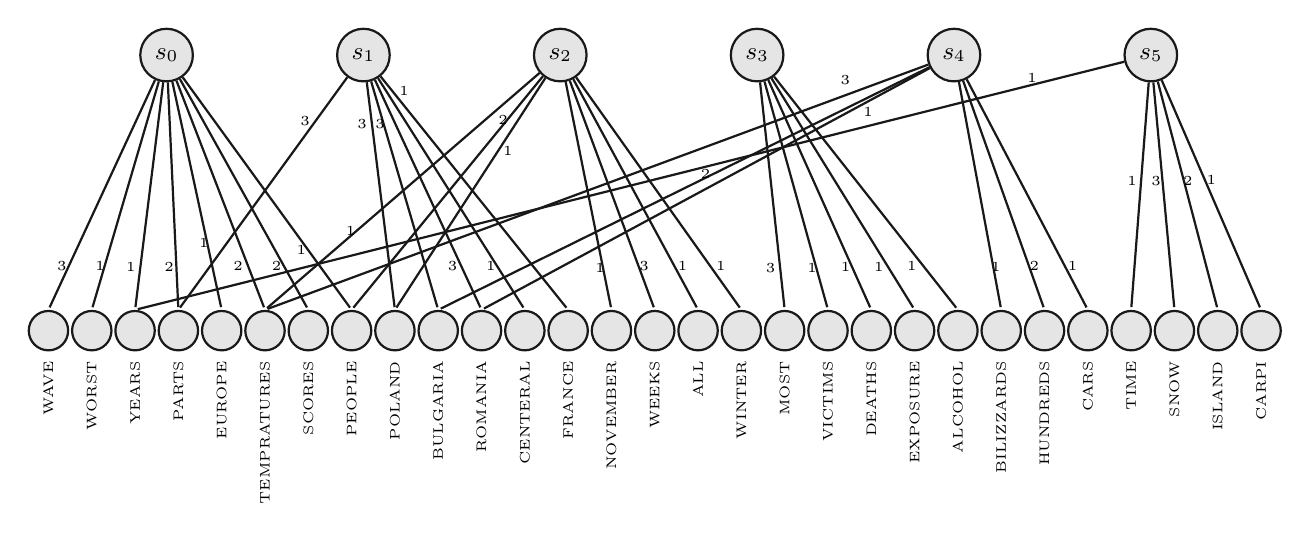
\begin{tikzpicture}[shorten >=1pt,-,scale=0.5]  
		\tikzstyle{sentence}=[circle,thick,draw=black!90,fill=black!10,minimum size=2mm]
	\tikzstyle{entity}=[circle,thick,draw=black!90,fill=black!10,minimum size=5mm]
		\tikzstyle{edge}=[draw=black!90, thick]
	   \begin{scope}
	   
		 \node [sentence] (s0) at (-3,0) {\small{$s_0$}};
		 \node [sentence] (s1) at (2,0) {\small{$s_1$}};
		 \node [sentence] (s2) at (7,0) {\small{$s_2$}}; 
		 \node [sentence] (s3) at (12,0) {\small{$s_3$}}; 
		 \node [sentence] (s4) at (17,0) {\small{$s_4$}};
		 \node [sentence] (s5) at (22,0) {\small{$s_5$}}; 
		 


	 \node [entity, label=below:\rotatebox{+90}{\tiny{WAVE}}] (e0)  at (-6.0,-7) {}; 
	 \node [entity, label=below:\rotatebox{+90}{\tiny{WORST}}] (e1)  at (-4.9,-7) {};
	 \node [entity, label=below:\rotatebox{+90}{\tiny{YEARS}}] (e2)  at (-3.8,-7) {}; 
	 \node [entity, label=below:\rotatebox{+90}{\tiny{PARTS}}] (e3)  at (-2.7,-7) {}; 
	 \node [entity, label=below:\rotatebox{+90}{\tiny{EUROPE}}] (e4)  at (-1.6,-7) {}; 
	 \node [entity, label=below:\rotatebox{+90}{\tiny{TEMPRATURES}}] (e5)  at (-0.5,-7) {}; 
	 \node [entity, label=below:\rotatebox{+90}{\tiny{SCORES}}] (e6)  at (0.6,-7) {}; 
	 \node [entity, label=below:\rotatebox{+90}{\tiny{PEOPLE}}] (e7)  at (1.7,-7) {}; 
	 \node [entity, label=below:\rotatebox{+90}{\tiny{POLAND}}] (e8)  at (2.8,-7) {}; 
	 \node [entity, label=below:\rotatebox{+90}{\tiny{BULGARIA}}] (e9)  at (3.9,-7) {}; 
	 \node [entity, label=below:\rotatebox{+90}{\tiny{ROMANIA}}] (e10)  at (5.0,-7) {}; 
	 \node [entity, label=below:\rotatebox{+90}{\tiny{CENTERAL}}] (e11)  at (6.1,-7) {}; 
	 \node [entity, label=below:\rotatebox{+90}{\tiny{FRANCE}}] (e12)  at (7.2,-7) {}; 
	 \node [entity, label=below:\rotatebox{+90}{\tiny{NOVEMBER}}] (e13)  at (8.3,-7) {}; 
	 \node [entity, label=below:\rotatebox{+90}{\tiny{WEEKS}}] (e14)  at (9.4,-7) {}; 
	 \node [entity, label=below:\rotatebox{+90}{\tiny{ALL}}] (e15)  at (10.5,-7) {}; 
	 \node [entity, label=below:\rotatebox{+90}{\tiny{WINTER}}] (e16)  at (11.6,-7) {}; 
	 \node [entity, label=below:\rotatebox{+90}{\tiny{MOST}}] (e17)  at (12.7,-7) {}; 
	 \node [entity, label=below:\rotatebox{+90}{\tiny{VICTIMS}}] (e18)  at (13.8,-7) {}; 
	 \node [entity, label=below:\rotatebox{+90}{\tiny{DEATHS}}] (e19)  at (14.9,-7) {}; 
	 \node [entity, label=below:\rotatebox{+90}{\tiny{EXPOSURE}}] (e20)  at (16.0,-7) {}; 
	 \node [entity, label=below:\rotatebox{+90}{\tiny{ALCOHOL}}] (e21)  at (17.1,-7) {}; 
	 \node [entity, label=below:\rotatebox{+90}{\tiny{BILIZZARDS}}] (e22)  at (18.2,-7) {}; 
	 \node [entity, label=below:\rotatebox{+90}{\tiny{HUNDREDS}}] (e23)  at (19.3,-7) {}; 
	 \node [entity, label=below:\rotatebox{+90}{\tiny{CARS}}] (e24)  at (20.4,-7) {}; 
	 \node [entity, label=below:\rotatebox{+90}{\tiny{TIME}}] (e25)  at (21.5,-7) {}; 
	 \node [entity, label=below:\rotatebox{+90}{\tiny{SNOW}}] (e26)  at (22.6,-7) {}; 
	 \node [entity, label=below:\rotatebox{+90}{\tiny{ISLAND}}] (e27)  at (23.7,-7) {}; 
	 \node [entity, label=below:\rotatebox{+90}{\tiny{CARPI}}] (e28)  at (24.8,-7) {}; 

		 
	 \path[edge] (s0) edge [above, very near end] node[font=\tiny] {$3$} (e0.north); %, line width=0.3ex
	 \path[edge] (s0) edge [above, very near end] node[font=\tiny] {$1$} (e1.north);
	 \path[edge] (s0) edge [above, very near end] node[font=\tiny, xshift=-1mm] {$1$} (e2.north);
	 \path[edge] (s0) edge [above, very near end] node[font=\tiny, xshift=-1mm] {$2$} (e3.north);
	 \path[edge] (s0) edge [above, very near end] node[font=\tiny, yshift=3mm, xshift=-1.5mm] {$1$} (e4.north);
	 \path[edge] (s0) edge [above, very near end] node[font=\tiny, xshift=-2mm] {$2$} (e5.north);
	 \path[edge] (s0) edge [above, very near end] node[font=\tiny, xshift=-2mm] {$2$} (e6.north);
	 \path[edge] (s0) edge [above, very near end] node[font=\tiny, yshift=2mm, xshift=-3.7mm] {$1$} (e7.north);

	 \path[edge] (s1) edge [above, near start] node[font=\tiny, near start] {$3$} (e3.north);
	 \path[edge] (s1) edge [above, near start] node[font=\tiny, xshift=-1.5mm] {$3$} (e8.north);
	 \path[edge] (s1) edge [above, near start] node[font=\tiny, xshift=-1mm] {$3$} (e9.north);
	 \path[edge] (s1) edge [above, very near end] node[font=\tiny, xshift=-2mm] {$3$} (e10.north);
	 \path[edge] (s1) edge [above, very near end] node[font=\tiny, xshift=-2mm] {$1$} (e11.north);
	 \path[edge] (s1) edge [above, very near start] node[font=\tiny] {$1$} (e12.north);

	 \path[edge] (s2) edge [above, very near end] node[font=\tiny, yshift=4.4mm, xshift=6.5mm] {$1$} (e5.north);
	 \path[edge] (s2) edge [above, near start] node[font=\tiny, xshift=1mm] {$2$} (e7.north);
	 \path[edge] (s2) edge [below, near start] node[font=\tiny] {$1$} (e8.north);
	 \path[edge] (s2) edge [below,  near end] node[font=\tiny] {$1$} (e13.north);
	 \path[edge] (s2) edge [above, very near end] node[font=\tiny] {$3$} (e14.north);
	 \path[edge] (s2) edge [above, very near end] node[font=\tiny] {$1$} (e15.north);
	 \path[edge] (s2) edge [above, very near end] node[font=\tiny] {$1$} (e16.north);

	 \path[edge] (s3) edge [below,  near end] node[font=\tiny,xshift=-1mm] {$3$} (e17.north);
	 \path[edge] (s3) edge [below,  near end] node[font=\tiny] {$1$} (e18.north);
	 \path[edge] (s3) edge [below,  near end] node[font=\tiny] {$1$} (e19.north);
	 \path[edge] (s3) edge [below,  near end] node[font=\tiny] {$1$} (e20.north);
	 \path[edge] (s3) edge [below,  near end] node[font=\tiny] {$1$} (e21.north);

	 \path[edge] (s4) edge [above, very near start] node[font=\tiny] {$3$} (e5.north);
	 \path[edge] (s4) edge [below, very near start] node[font=\tiny] {$1$} (e9.north);
	 \path[edge] (s4) edge [above, midway] node[font=\tiny] {$2$} (e10.north);
	 \path[edge] (s4) edge [above, very near end] node[font=\tiny] {$1$} (e22.north); 
	 \path[edge] (s4) edge [above, very near end] node[font=\tiny] {$2$} (e23.north); 
	 \path[edge] (s4) edge [above, very near end] node[font=\tiny] {$1$} (e24.north);     

	 \path[edge] (s5) edge [above, very near start] node[font=\tiny, xshift=4mm] {$1$} (e2.north);
	 \path[edge] (s5) edge [above, midway] node[font=\tiny,xshift=-1mm] {$1$} (e25.north);
	 \path[edge] (s5) edge [above, midway] node[font=\tiny,xshift=-1mm] {$3$} (e26.north);
	 \path[edge] (s5) edge [above, midway] node[font=\tiny] {$2$} (e27.north); 
	 \path[edge] (s5) edge [above, midway] node[font=\tiny] {$1$} (e28.north);    
		\end{scope}        
	  \end{tikzpicture}
\end{tabular}
\caption{The entity graph representation of the text in Table \ref{}.}
\label{f:entity_graph}
\end{figure}



Figure \ref{f:entity_graph} shows how a bipartite graph captures the distribution of entities between sentences of a text. 


\subsection{Coherence Representation: Average Outdegree of Projection Graphs}
%
Coherence is almost about the connectivity of sentences of a text. 
Sentences are modeled as, just, one set of nodes in the entity graph representation.  
In graph theory, there are different ways to project a bipartite graph, which consists of two sets of nodes, into a graph whose nodes are only one set of nodes of the bipartite graph. 
This graph is called one-mode projection graph and its edges are obtained based on the other set of nodes of the bipartite graph. 
One-mode projection graphs can be weighted in different ways in order to retain the information of the bipartite graph. 


\newcite{guinaudeau13} apply one-mode projection \cite{newmanmark10} to the sentence nodes of the bipartite graph to represent the connections that exist between –- potentially non adjacent –- sentences in the graph. 
These projections result in graphs where nodes correspond to sentences and an edge is created between two nodes if the corresponding sentence node in the bipartite graph have at least one entity in common. 
Contrary to the bipartite graph, edges in one-mode projections are directed representing the order of sentences in texts. 



\newcite{guinaudeau13} apply three kinds of projections, $P_U$, $P_W$ and $P_{Acc}$, depending on
the weighting scheme associated with their edges. 
In, $P_U$, weights are binary and equal to $1$ where two sentences have a least one entity in common. 
This projection graph only shows the which sentences are linked to each other based on entity relations. 
In $P_W$, edges are weighted according to the number of entities ``shared” by two sentences. 
This projection graph is more informative than $P_U$ so that sentence nodes that are adjacent to more entity nodes in a bipartite graph are more strongly connected than those with less common entity nodes. 
In $P_{Acc}$ syntactic information is accounted for by integrating the edge weights in the bipartite graph. 
In this case, weights are equal to

\begin{equation}
W_{ik} = \sum_{e \in E_{ik}}{w(e,s_i) \cdot w(e,s_k)}
\end{equation}


where $E_{ik}$ is the set of entities shared by $s_i$ and $s_k$. 
This type of the projection graph is more informative than two others in this sense that it incorporate the grammatical information, which are roughly similar to syntactical transitions in the entity grid model, as weight of edges. 
Figure \ref{} shows $P_U$, $P_W$, and $P_{Acc}$ graphs obtained from the presented bipartite graph in Figure \ref{}.


\begin{figure}[!t]
\centering
\small

% \begin{tabular}{lc}

% \begin{tikzpicture}        
% 		 \node [] (n0) at (0,0) {};
%          \node [] (label) at (0,0.8) {$P_U:$};
% \end{tikzpicture}
% &
% \begin{tikzpicture}[shorten >=1pt,->,scale=0.5]  
%         \tikzstyle{sentence}=[circle,thick,draw=black!90,fill=black!10,minimum size=2mm]
% 		\tikzstyle{entity}=[circle,thick,draw=black!90,fill=black!10,minimum size=2mm]
%         \tikzstyle{edge}=[draw=black!90, thick]

%        \begin{scope}
       
%          \node [sentence] (s0) at (0,0) {\tiny{$s_0$}};
%          \node [sentence] (s1) at (3,0) {\tiny{$s_1$}};
%          \node [sentence] (s2) at (6,0) {\tiny{$s_2$}}; 
%          \node [sentence] (s3) at (9,0) {\tiny{$s_3$}}; 
%          \node [sentence] (s4) at (12,0) {\tiny{$s_4$}};
%          \node [sentence] (s5) at (15,0) {\tiny{$s_5$}}; 
 
%  		\path[edge] (s0) edge [above] node[font=\tiny]{} (s1);
%  		\path[edge, bend left = 30] (s0) edge [above] node[font=\tiny]{} (s2);
% 		\path[edge, bend left = 30] (s0) edge [above] node[font=\tiny]{} (s4);
%  		\path[edge, bend left = 30] (s0) edge [above] node[font=\tiny]{} (s5);

%  		\path[edge] (s1) edge [above] node[font=\tiny]{} (s2);
% 		\path[edge, bend right = 30] (s1) edge [above] node[font=\tiny]{} (s4);
           
%         \end{scope}        
%       \end{tikzpicture}

% \\

% \begin{tikzpicture}        
% 		 \node [] (n0) at (0,0) {};
%          \node [] (label) at (0,0.8) {$P_W:$};
% \end{tikzpicture}
%  &
% \begin{tikzpicture}[shorten >=1pt,->,scale=0.5]  
%         \tikzstyle{sentence}=[circle,thick,draw=black!90,fill=black!10,minimum size=2mm]
% 		\tikzstyle{entity}=[circle,thick,draw=black!90,fill=black!10,minimum size=2mm]
%         \tikzstyle{edge}=[draw=black!90, thick]

%        \begin{scope}
       
%          \node [sentence] (s0) at (0,0) {\tiny{$s_0$}};
%          \node [sentence] (s1) at (3,0) {\tiny{$s_1$}};
%          \node [sentence] (s2) at (6,0) {\tiny{$s_2$}}; 
%          \node [sentence] (s3) at (9,0) {\tiny{$s_3$}}; 
%          \node [sentence] (s4) at (12,0) {\tiny{$s_4$}};
%          \node [sentence] (s5) at (15,0) {\tiny{$s_5$}}; 
 
%  		\path[edge                ] (s0) edge [above, midway] node[font=\tiny]{$1$} (s1);
%  		\path[edge, bend left = 30] (s0) edge [above, near end] node[font=\tiny]{$2$} (s2);
% 		\path[edge, bend left = 30] (s0) edge [above, near end] node[font=\tiny]{$1$} (s4);
%  		\path[edge, bend left = 30] (s0) edge [above, midway] node[font=\tiny]{$1$} (s5);

%  		\path[edge                 ] (s1) edge [above, midway] node[font=\tiny]{$1$} (s2);
% 		\path[edge, bend right = 30] (s1) edge [above, midway] node[font=\tiny]{$2$} (s4);
           
%         \end{scope}        
%       \end{tikzpicture}

% \\

% \begin{tikzpicture}        
% 		 \node [] (n0) at (0,0) {};
%          \node [] (label) at (0,0.8) {$P_{Acc}:$};
% \end{tikzpicture}
%  &
%    \begin{tikzpicture}[shorten >=1pt,->,scale=0.5]  
%         \tikzstyle{sentence}=[circle,thick,draw=black!90,fill=black!10,minimum size=2mm]
% 		\tikzstyle{entity}=[circle,thick,draw=black!90,fill=black!10,minimum size=2mm]
%         \tikzstyle{edge}=[draw=black!90, thick]

%        \begin{scope}
       
%          \node [sentence] (s0) at (0,0) {\tiny{$s_0$}};
%          \node [sentence] (s1) at (3,0) {\tiny{$s_1$}};
%          \node [sentence] (s2) at (6,0) {\tiny{$s_2$}}; 
%          \node [sentence] (s3) at (9,0) {\tiny{$s_3$}}; 
%          \node [sentence] (s4) at (12,0) {\tiny{$s_4$}};
%          \node [sentence] (s5) at (15,0) {\tiny{$s_5$}}; 
 
%  		\path[edge                ] (s0) edge [above, midway] node[font=\tiny]{$6$} (s1);
%  		\path[edge, bend left = 30] (s0) edge [above, near end] node[font=\tiny]{$4$} (s2);
% 		\path[edge, bend left = 30] (s0) edge [above, near end] node[font=\tiny]{$6$} (s4);
%  		\path[edge, bend left = 30] (s0) edge [above, midway] node[font=\tiny]{$1$} (s5);

%  		\path[edge                 ] (s1) edge [above, midway] node[font=\tiny]{$3$} (s2);
% 		\path[edge, bend right = 30] (s1) edge [above, midway] node[font=\tiny]{$9$} (s4);
           
%         \end{scope}        
%       \end{tikzpicture}

% \end{tabular}
% \caption{$P_U$, $P_W$, and $P_{Acc}$ projection graphs.}

% \label{f:entity_projection}
% \end{figure}


Distance between sentences can be integrated in the weight of the one-mode projection graphs to decrease the importance of links that exist between nonadjacent sentences. 
In this case, the weights of the projection graphs are divided by the number of sentences in between of two sentences. 

Inspired from the centrality measure in graph theory that measures the connectivity of nodes in a graph, the coherence of a text can be measured by computing the average outdegree of a projection graph as follow:

\begin{equation}
Coh(T) = AvgOutDeg(P) = \frac{1}{N} \sum_{\textit{i \ in 1..N}} outDegree(s_i),
\end{equation}

where $outdegree(s_i)$ is the sum of the weights associated to edges that leave $s_i$ and $N$ is the number of nodes in graph $P$. 

In our running example the average outdegrees in different projection graphs are as follows:

% \begin{table}[!ht]
% \centering
% \begin{tabular}{l|l}
% \hline
%  $P$ & $ AvgOutDeg(P) = Coh(T)$ \\\hline
%  $P_U$ & $\frac{1}{6} \left((1+1+1+1)+(1+1)+(0)+(0)+(0)+(0)) \right) = 1.00$ \\
%  $P_W$ & $\frac{1}{6} \left((1+2+1+1)+(1+2)+(0)+(0)+(0)+(0)) \right) = 1.33$\\
%  $P_{Acc}$ &$\frac{1}{6} \left((6+4+6+1)+(3+9)+(0)+(0)+(0)+(0)) \right) = 4.83$ \\
%  $P_U\textit{, }Dist$ & $\frac{1}{6} \left((1+0.50+0.25+0.20)+(1+0.33)+(0)+(0)+(0)+(0)) \right) = 0.55$ \\
%  $P_W\textit{, }Dist$ & $\frac{1}{6} \left((1+1+0.25+0.20)+(1+0.66)+(0)+(0)+(0)+(0)) \right)= 0.69$ \\
%  $P_{Acc}\textit{, }Dist$ & $\frac{1}{6} \left((6+2+1.5+0.2)+(3+3)+(0)+(0)+(0)+(0)) \right)= 2.61$ \\ \\
%  \hline
% \end{tabular}
% \end{table}

It is worth to mention that the proposed entity graph model by \newcite{guinaudeau13} is an unsupervised model meaning that the final average outdegree can be directly used for comparing two texts with respect to their coherence. 
\newcite{guinaudeau13} assume that projection graphs of coherent texts contain more edges than the projection graph of  incoherent texts. 
Therefore, the projection graph of coherent texts are expected to have higher average outdegree than the projection graph of incoherent texts.  
That is the intuition of using average outdegree as a metric that measures the connectivity of nodes in projection graphs and consequently the coherence of texts. 


\section{The Normalized Entity Graph Model}
%
\subsection{Motivation}
%
The entity graph model uses the projection graph representation of a text to measure its coherence. 
As discussed above, depending on how weights of edges in projection graphs are computed, different types of projection graphs can be proposed. 
Based on what information of the entity graph is critical to be transfered to projection graphs weights of the projection graphs are computed.
For example, $P_U$, which is the basic projection graph proposed by \newcite{guinaudeau13}, only captures this information of  entity graphs that if two sentence nodes have an entity node in common. 
$P_W$ is more informative and sets the number of common entities between two sentence nodes in the entity graph as a weight to the edge that connects those sentences nodes in the projection graph. 
$P_{Acc}$ incorporates grammatical transitions of common entities between sentence nodes of the entity graph in the process of weight calculation of edges of projection graphs. 


An important information that is used in the entity grid model but is missed in the entity graph model is the salience of entities. 
In the entity grid model the frequency of an entity\footnote{Frequency of an entity means the number of mentions of an entity in a text.} is considered an indicator of its importance. 
However, the importance of an entity in a sentence depends on many factors such as its syntactical role, the number of mentioned entities in that sentence, and etc. 
With this motivation we propose a new version of the entity graph model that takes into account the importance of entities and sentences based on the topology of the entity graph. 

The normalization is applied on weights of the entity graph and then one-mode projections. 
The normalization is based on the relative importance of entities and, in turn, the relative importance of sentences. 
Including negative information, such as the number of a sentence's entities that are not shared with other sentences, allows to normalize the importance of entities according to sentence length (measured in terms
of entity mentions), and hence to capture distance information between mentions of the same entity.
This brings the entity graph closer to \newcite{stoddard91,p.30} notion of cohesion: ``The relative cohesiveness of a text depends on the number of cohesive ties [...] and on the distance between the nodes and their associated cohesive elements.” By using this information, edge weights are set less arbitrary. 
Normalization also allows to include distance between mentions of the same entity.  

As it stated in \cite{zhoudengyong07,zweig11} that normalizing weights leads to better performance. 

\subsection{Text Representation: Normalized Entity Graph}
%
We employ the entity graph representation for modeling the distribution of entities over adjacent sentences. 
As a recall, this graph is weighted and the weight of each edge represents the grammatical role of each entity in each sentence.  


The definition of silence has two sides. 
One side is that salient entities are mentioned in important sentences.  
On the other side, important sentences contain salient entities and they are connected to each other because they share salient entities. 
That is why we approach to salience as a relative concept where the salience of an entity is computed with respect to other entities and sentences in a text. 

Our intuition is inspired by information retrieval where each sentence is supposed to carry a piece of information in a text. 
In entity-based coherence models, entities make information that is included in a sentence. 
When a sentence contains many entities it gets more difficult for a reader to process the expressed relation between entities in the sentence. 
This is roughly captured by readability formulas in that texts with long sentences are more difficult to read because they take more processing time of their readers. 
On the other hand, sentences that contain most entities that are mentioned in a text are more important than other sentences, because they contain most information of a text. 

Our normalization process defines a trade off between the above factors in a text.  
The normalization process consists of two main steps: how important is an entity for each individual sentence, and how important is a sentence for a text. 


Here we normalize the weights of mentioned entities in a sentence with respect to the weight of the rest of entities in the sentence. 
This takes negative information into account as entities which do not occur in other sentences also count. 
We follow \newcite{newmanmark10} by applying node degree normalization. 

Given an entity graph, the normalized weight of an edge that connect an entity node, $e$, to a sentence node, $s$, equals the current weight of that edge divided by the sum of weights of edges that are connected to the sentence node, $s$. 
This gives the importance of each entity in a sentence relative to the sentence’s other entities.

\begin{equation}
Imp(s,e) = \frac{w(s,e)}{\sum_{e^{`}\in Entities}{w(s,e^{`})}}.
\end{equation} 

Moreover, in order to compute the relative importance of sentences with respect to each other, we measure what portion of information in a text is present in each sentence. 
Since we are modeling local coherence, for any pair of sentences we compute their relative importance. 
Following \cite{rode08}, we use the following formula to compute the relative importance of each sentence:

\begin{equation}
w(s_i, s_j) = \frac{||s_i||}{||s_i|| + ||s_j ||},
\end{equation}

This value is equal to the degree of each sentence in the entity graph.  

\subsection{Coherence Representation: Normalized Projection Graph}
%
Similar to the entity graph model, we use the one-mode projection graph of the entity graph representation to encode the connections between sentences. 
Then we compute the average outdegree of nodes in projection graphs as a measure of coherence. 

Since $P_U$ is not weighted the normalization does not affect this projection graph. 

Above we explained how we normalize an entity graph. 
Since the grammatical roles of entities are not used in $P_w$,  we assume that the entity graph is unweighted. 
So the normalization process is just dividing the weight of each edge in the entity graph by the degree of the corresponding sentence node. 
If a sentence contains many entities, then the amount of information each entity contributes is reduced.
Assume $||s||$ as the number of entities in sentence $s$.  
The importance of entity $e$ for $s$ is 

\begin{equation}
Imp(s,e) = \frac{1}{||s||}.
\end{equation}

For $P_{Acc}$, we follow the normalization process as it is explained above. 
The entity graph model weighs edges by the number of entities sentences share ($P_W$) and which syntactic functions the entities occupy ($P_{Acc}$). 


Regardless of what type of projection graph we are building, the weight of the edge that connects sentences $s_i$ and $s_j$ is:

\begin{equation}
W(s_i,s_j) = \sum_{e \in E_i+E_j}{(w_{s_i}^{s_j}.Imp(s_i,e))+(w_{s_j}^{s_i}.Imp(s_j,e))}.
\end{equation}

Intuitively, the above equation computes the local coherence between any pair of sentences. 
Given a pair of sentences, the sentence that contains more entities is more informative and almost more important while the importance of entities in longer sentences are more discarded. 
Similar to \cite{rode08}, we use the product of $w_{s_i}^{s_j}$ and $Imp(s_i; e)$ to approximate the local salience of entity $e$ in each sentence $s_i$. 
This prevents the model to get biased by the length of sentences. 

Figure \ref{fig:normalized_entity_projection} depicts normalized version of the projection graphs presented in Figure \ref{}. 

% \begin{figure}[!t]
% \centering
% \begin{tabular}{lc}

% \begin{tikzpicture}        
% 		 \node [] (n0) at (0,0) {};
%          \node [] (label) at (0,0.8) {$P_U:$};
% \end{tikzpicture}
% &
% \begin{tikzpicture}[shorten >=1pt,->,scale=0.5]  
%         \tikzstyle{sentence}=[circle,thick,draw=black!90,fill=black!10,minimum size=2mm]
% 		\tikzstyle{entity}=[circle,thick,draw=black!90,fill=black!10,minimum size=2mm]
%         \tikzstyle{edge}=[draw=black!90, thick]

%        \begin{scope}
       
%          \node [sentence] (s0) at (0,0) {\tiny{$s_0$}};
%          \node [sentence] (s1) at (3,0) {\tiny{$s_1$}};
%          \node [sentence] (s2) at (6,0) {\tiny{$s_2$}}; 
%          \node [sentence] (s3) at (9,0) {\tiny{$s_3$}}; 
%          \node [sentence] (s4) at (12,0) {\tiny{$s_4$}};
%          \node [sentence] (s5) at (15,0) {\tiny{$s_5$}}; 
 
%  		\path[edge] (s0) edge [above] node[font=\tiny]{} (s1);
%  		\path[edge, bend left = 30] (s0) edge [above] node[font=\tiny]{} (s2);
% 		\path[edge, bend left = 30] (s0) edge [above] node[font=\tiny]{} (s4);
%  		\path[edge, bend left = 30] (s0) edge [above] node[font=\tiny]{} (s5);

%  		\path[edge] (s1) edge [above] node[font=\tiny]{} (s2);
% 		\path[edge, bend right = 30] (s1) edge [above] node[font=\tiny]{} (s4);
           
%         \end{scope}        
%       \end{tikzpicture}

% \\

% \begin{tikzpicture}        
% 		 \node [] (n0) at (0,0) {};
%          \node [] (label) at (0,0.8) {$P_W:$};
% \end{tikzpicture}
%  &
% \begin{tikzpicture}[shorten >=1pt,->,scale=0.5]  
%         \tikzstyle{sentence}=[circle,thick,draw=black!90,fill=black!10,minimum size=2mm]
% 		\tikzstyle{entity}=[circle,thick,draw=black!90,fill=black!10,minimum size=2mm]
%         \tikzstyle{edge}=[draw=black!90, thick]

%        \begin{scope}
       
%          \node [sentence] (s0) at (0,0) {\tiny{$s_0$}};
%          \node [sentence] (s1) at (3,0) {\tiny{$s_1$}};
%          \node [sentence] (s2) at (6,0) {\tiny{$s_2$}}; 
%          \node [sentence] (s3) at (9,0) {\tiny{$s_3$}}; 
%          \node [sentence] (s4) at (12,0) {\tiny{$s_4$}};
%          \node [sentence] (s5) at (15,0) {\tiny{$s_5$}}; 
 
%  		\path[edge                ] (s0) edge [above, midway] node[font=\tiny]{$\frac{2}{14}$} (s1);
%  		\path[edge, bend left = 30] (s0) edge [above, near end] node[font=\tiny]{$\frac{4}{15}$} (s2);
% 		\path[edge, bend left = 30] (s0) edge [above, near end] node[font=\tiny]{$\frac{2}{14}$} (s4);
%  		\path[edge, bend left = 30] (s0) edge [above, midway] node[font=\tiny]{$\frac{2}{13}$} (s5);

%  		\path[edge                 ] (s1) edge [above, midway] node[font=\tiny]{$\frac{2}{13}$} (s2);
% 		\path[edge, bend right = 30] (s1) edge [above, midway] node[font=\tiny]{$\frac{4}{12}$} (s4);
           
%         \end{scope}        
%       \end{tikzpicture}

% \\

% \begin{tikzpicture}        
% 		 \node [] (n0) at (0,0) {};
%          \node [] (label) at (0,0.8) {$P_{Acc}:$};
% \end{tikzpicture}
%  &
%    \begin{tikzpicture}[shorten >=1pt,->,scale=0.5]  
%         \tikzstyle{sentence}=[circle,thick,draw=black!90,fill=black!10,minimum size=2mm]
% 		\tikzstyle{entity}=[circle,thick,draw=black!90,fill=black!10,minimum size=2mm]
%         \tikzstyle{edge}=[draw=black!90, thick]

%        \begin{scope}
       
%          \node [sentence] (s0) at (0,0) {\tiny{$s_0$}};
%          \node [sentence] (s1) at (3,0) {\tiny{$s_1$}};
%          \node [sentence] (s2) at (6,0) {\tiny{$s_2$}}; 
%          \node [sentence] (s3) at (9,0) {\tiny{$s_3$}}; 
%          \node [sentence] (s4) at (12,0) {\tiny{$s_4$}};
%          \node [sentence] (s5) at (15,0) {\tiny{$s_5$}}; 
 
%  		\path[edge                ] (s0) edge [above, midway] node[font=\tiny]{$.180$} (s1);
%  		\path[edge, bend left = 30] (s0) edge [above, near end] node[font=\tiny]{$.223$} (s2);
% 		\path[edge, bend left = 30] (s0) edge [above, near end] node[font=\tiny]{$.216$} (s4);
%  		\path[edge, bend left = 30] (s0) edge [above, midway] node[font=\tiny]{$.095$} (s5);

%  		\path[edge                 ] (s1) edge [above, midway] node[font=\tiny]{$.153$} (s2);
% 		\path[edge, bend right = 30] (s1) edge [above, midway] node[font=\tiny]{$.314$} (s4);
           
%         \end{scope}        
%       \end{tikzpicture}

% \end{tabular}
% \caption{$P_U$, $P_W$, and $P_{Acc}$ normalized projection graphs.}
% \label{fig:normalized_entity_projection}
% \end{figure}


Table \ref{} shows the outdegree of each projection graph. 


\section{Experiments}
%
In this section, we compare the introduced local coherence models (i.e., the entity graph model, the entity grid model, and the normalized entity graph model) in three benchmark tasks: sentence ordering, summary coherence ranking, and readability assessment. 
We show that although the entity graph model is an unsupervised model, it outperforms the entity grid model (as a supervised model) on these tasks. 
This shows that graphs are a suitable framework to model coherence of a text. 
We evaluate our proposed normalization on the entity graph model and show that our normalized entity graph model obtains a higher performance than the entity graph model. 
This indicates that the entity graph model is a good framework but it is far away from perfect and can be improved.  
The results of our experiments in this chapter motive us to consider the entity graph representation of texts for developing new coherence features and model. 


% We compare the normalized entity graph with the entity graph on all tasks, Guinaudeau and Strube
% (2013) compared their work with the entity grid (Barzilay and Lapata, 2008; Elsner and Charniak,
% 2011): sentence ordering, summary coherence rating and readability assessment. 
% Following Guinaudeau and Strube (2013) we test statistical significance with the Student’s t-test and Bonferroni
% correction, to check whether the best result (bold value in the tables) is significantly different from
% the results of the entity graph and the normalized entity graph. 
% Diacritics ** indicate significance level 0.01, * indicates significance level 0.05.

\subsection{Sentence Ordering}
%
It is known that the order of information in coherent texts is such that they are easy to follow \cite{lapata03,barzilay04,karamanis04b,barzilay05a,soricut06}. 
As it is explained in the definition of coherence, a text is more than a random concatenation of sentences;
the order of sentences affects how difficult the presented information in a text can be understood, if at all. 
Given the above fact, a document can be taken as an unordered bag of sentences and the task would be to find the ordering of the sentences that maximizes coherence according to a model. 
Unfortunately, finding the best ordering is NP-complete \cite{?} and non-approximable \cite{althaus04}.
Therefore, this task need to be simplified to be used for coherence evaluation. 
Two restricted versions of the sentence ordering tasks are the discrimination task, and the insertion task. 
In both subtasks we evaluate whether our model is able to distinguish between the correct (original) order of sentences in a document and an incorrect (non-original) one. 

\subsubsection{Discrimination}
%
The discrimination task is based on this fact that the original order of sentences in a document is taken as the best order and any scrambling of sentences disturbs the perceived coherence of the document. 
Therefore, by rearranging the order of sentences of a document, we are making the document more difficult to understand or less coherent, because the order of presented information is disturbed. 

More formally, let $COH_M(d)$ be the coherence estimation of document $d$ by the coherence model $M$ and $p$ be a version of $d$ that its sentences are randomly permuted, then the coherence model $M$ should ideally distinguish document $d$ a more coherent document than $p$:

\begin{equation}
COH_M(d) > COH_M(p). 
\end{equation}


\paragraph{Setting}
%
We use the same setting that is used in \newcite{guinaudeau13}. 
$61$ documents are extracted from the English test part of the CoNLL $2012$ shared task \cite{pradhan12}. 
Documents are composed of $36.1$ sentences and $2064$ word tokens on average. 

In this experiment, a model associates local coherence values with the original document and its permutation, if the score for the original order of sentences of a document is higher than the score of the permutation version of sentence then the output of our system being considered correct. 

We use $20$ permutations of each text. 
Because we do not know the relative quality of different permutations, the dataset includes only pairwise rankings that comprise the original document and one of its permutations.

We employ two evaluation metrics: accuracy and F-measure. 
Accuracy is used to evaluate how correctly a coherence model discriminates the original order of a document from its $20$ different permutations.
It equals the number of times the model gives a higher score to the original document than the score that it gives to a permutation, divided by the number of comparisons.

\begin{equation}
Acc  = \frac{\#\textit{ of correct predictions}}{\#\textit{ of comparisons}}
\end{equation}

We also computed F-measure because the model may give the same score to a permutation and the original document. 
In order to compute F-measure, we need to compute recall and precision as follow:

\begin{equation}
recall = \frac{correct}{total},
\end{equation}
where $total$ is the total number of test samples no matter if on them the model can make a decision or not. 

\begin{equation}
precision = \frac{correct}{decisions},
\end{equation}
where $decision$ is the number of samples on that the model made a decision.

\begin{equation}
F1 = 2.\frac{precision \cdot recal}{precision + recall}
\end{equation}


We test significance by the Student’s t-test that detects statistically significant differences between paired samples.
Moreover, as increasing the number of hypotheses in a test can also increase the likelihood of witnessing a rare event, and therefore, the chance to reject the null hypothesis when it is true, we use the Bonferroni correction to adjust the increased
random likelihood of apparent significance. 

In contrast the entity graph model, the entity grid model is a supervised model. 
The above setting makes it easy to define a machine learning setup for the entity grid model. 
Following \newcite{barzilay08}, if we assume that the $COH_M(d)$ is a linear function of coherence features, which are defined as the entity transitions in the entity grid model as follows:

\begin{equation}
COH_M(d) = \vec{w}^{T}.\vec{t}
\end{equation}

where $w$ is a vector of parameters and $t$ is the feature vector representing the coherence of $d$. 
The goal of the learning procedure is learn the best values for parameters $w$ in order to minimize the number of violations of pairwise rankings provided in the training set:

\begin{equation}
COH_M(d) > COH_M(p)
\end{equation}

The problem typically treated as a Support Vector Machine (SVM) constraint optimization problem, and can be solved using the search technique implemented in $SVM_{ligh}$\footnote{link to the package} \cite{joachims02} package. 

Similar to \newcite{guinaudeau13} we do not use the ACCIDENTS and EARTHQUAKES datasets that are employed in the entity grid model. 
\newcite{guinaudeau13}'s main reason is that, as  it is also mentioned by \newcite{elsner08b}, the ACCIDENTS and EARTHQUAKES datasets use a very constrained style and are not typical of normal informative documents. 


For entity extractions all nouns in a document are considered discourse entities, even those that do not head NPs.
Nouns and grammatical information associated with each entity is extracted automatically thanks to the Stanford parser \cite{marneffe06} and Brown Coherence Toolkit \footnote{\url{https://bitbucket.org/melsner/}}. 



Results for \newcite{guinaudeau13}, G\&S, are reproduced, results for 
B\&L \newcite{barzilay08}, and E\&C \newcite{elsner11b},  are reported from \newcite{guinaudeau13}. 


\begin{table}[!t]
\centering
\begin{small}
\begin{tabular}{l|cc@{}l}
& Acc & F &\\\hline
Random & 0.496 & 0.496 & \\
B\&L & 0.877 & 0.877 &\\ 
E\&C & 0.915 & 0.915  &\\\hline

& \multicolumn{3}{|c}{Entity graph, G\&S} \\\hline 
$P_U$, \textit{Dist} & 0.830 & 0.830 & ** \\
$P_W$, \textit{Dist} & 0.871 & 0.871& \\
$P_{Acc}$, \textit{Dist} & 0.889 & 0.889& \\\hline

& \multicolumn{3}{|c}{Normalized entity graph} \\\hline 
$P_U$, \textit{Dist} & 0.830 & 0.830& ** \\
$P_W$, \textit{Dist} & 0.886 & 0.886&\\
$P_{Acc}$, \textit{Dist} & \textbf{0.909} & \textbf{0.909}&\\
\end{tabular}
\end{small}
\caption{Discrimination: baselines and entity graph vs.\ normalized
  entity graph}\label{t:exp1:sentence_ordering}  
\end{table}
%
In this experiment, the distance factor is crucial for the entity graph model and its normalized version. 
unlike the entity grid model, these two models do not incorporate the order of grammatical transitions. 
For instance, both transitions $S O$ and $O S$ yield the same edge weight, $6$, in the weighted projection graph, $P_{Acc}$. 
Moreover, an original document and its permutations contain the same entities. 
So without the distance factor these two models cannot distinguish between a document and its permutation. 
Intuitively, distance can model if sentences that share entities are located near to each other in a document or not. 
This is expected from coherent texts that neighboring sentences be about similar topics and therefore information of these sentences would be similar. 

The unweighted graph, $P_U$ is not weighted and it does not need any normalization.  
Hence the results for the entity graph and the normalized entity graph are identical.
Both are better than the Random baseline and worse than the performance of the B\&L model.
However, this projection graph is less informative than the B\&L model. 
Normalization improves the results for the weighted graphs $P_W$ and $P_{Acc}$ with $P_{Acc}$ outperforming B\&L
considerably and closely approaching E\&L. 
The results of this experiment show that our normalization model can transfer more information about the entity graph representation of a text to its projection graphs and improves the performance of the original entity graph model. 

The $P_{Acc}, Dist$ setting does not outperform E\&C model. 
It is important to note that the E\&C model is a supervised model and during training the model tunes the associated weights with entity transitions in order to obtain a better performance. 
In contrast, the entity graph model is an unsupervised model and its procedure is the same for any domain and task. 
Obtaining a competitive result near to a supervised model is promising.  


As we can see the performance of examined coherence models on the discrimination task are already high. 
It is mainly because the discrimination task can be easily solved without any notions of coherence. 
Discrimination specially becomes easier for longer documents, since the average random permutation grows less similar to the original document. 
The insertion task, the second related task to sentence ordering, somewhat overcomes this easiness. 


\subsubsection{Insertion}
%
Similar to the discrimination task, the insertion task \cite{chenerdong07} is designed to evaluate the ability of a coherence model in distinguishing the proper order of sentences in a document from the other orders. 
As we discussed, especially for documents with many sentences, permuting whole sentences yields a version of document that is very different, and therefore easier to distinguish, from the original document. 

The intuition behind the insertion task is that given a document where one of its sentences is removed, the perceived coherence 
of the document is discarded. 
A coherence model should be able to assign a higher coherence score to a permutation in that the removed sentence is located in its original position. 

Given a document with $n$ sentences, if the sentence at position $i$ is removed then there are $n$ possible positions, including the position $i$, to reinsert this sentence and create a permutation of this document. 
Table \ref{table:insertion_task} shows an example of removing the sentence in position $0$ ($\underline{A}$) of a document with four sentences, $\left \{ A, B, C, D \right \}$, and reinserting the sentence in all possible positions. 
 

\begin{table}[!ht]
\centering
\begin{small}
\begin{tabular}{cc|cccc}
position & original document  & \multicolumn{4}{c}{permutations}\\
\hline
$0$ & $\underline{A}$ & $\underline{A}$ & $B$ & $B$ & $B$\\
$1$ & $B$ 			  & $B$  & $\underline{A}$ & $C$ & $C$\\
$2$ & $C$			  & $C$ & $C$ & $\underline{A}$ & $D$\\
$3$ & $D$			  & $D$ & $D$ & $D$ & $\underline{A}$\\
\end{tabular}
\end{small}
\caption{}
\label{table:insertion_task}  
\end{table}

Besides any practical applications, insertion has two properties that make it well-suited for evaluation of coherence models. 
First, a document with $n$ sentences can be evaluated exactly in $n^2$ time, which, though it can be significant, is
still much faster than ordering and does not involve a potentially error-prone search.
Second, it grows more difficult as documents lengthen because permutations only differ by one sentence, unlike discrimination, which grow easier. 
Third, a document is compared to many more permutations in insertion task than in discrimination. 


For evaluation, we employ two evaluation metrics: accuracy and the insertion score (Ins.). 
Accuracy measures for how many sentences, out of the all sentences of a document, a coherence model exactly predicts the original position of the sentence as the best point to reinsert it. 
%(We report the average proportion of correct insertions per document.)
Therefore the accuracy is computed as follows:

\begin{equation}
Acc = \frac{1}{D}\sum_{d \in D}\frac{\#\textit{ of correctly placed sentences in d}}{\#\textit{ of sentences in d}}
\end{equation}
%
where $D$ is the set of documents in a dataset.  
By averaging over over documents, longer documents do not disproportionally influence the results. 

In complement to accuracy, we use the insertion score introduced by 
\newcite{elsner11b} for evaluation. 
This score  –- the higher, the better –-  is a positional score that measures how far the predicted position of a sentence by a coherence model is from the original position of the sentence. 
For each document this score is normalized by the length of document to be unbiased to the number of sentences in a document. 

More formally, this score is computed as follows:
\begin{equation}
Ins. = 1 - \frac{o - p}{norm(N, p)},
\end{equation}


\begin{equation}
norm(N, p) = \frac{1}{2*N} (p * (p-1) + (N - p + 1)*(N - p)),
\end{equation}
%
where $o$ and $p$ are respectively the original position of a removed sentence and its proposed position by the model. 
$N$ is the number of sentences in a document.  

We follow the same dataset that is used in the discrimination task.  
The system output is considered correct if the document associated with the highest local coherence score is
the one in which the sentence is reinserted in the correct position. 

We define a heuristic baseline to compare our models with. 
Since for a document with $n$ sentences, each sentence insertion is an n-way decision, a random baseline is expected that decision are sampled from an uniform distribution. 
For example for a document with two sentences, the probability of randomly predicting correctly is $50\%$. 
Thus, the random performance scales as $\frac{1}{n}$, going to zero as length increases.

\begin{table}[!b]
\centering
\begin{small}
\begin{tabular}{l|c@{}lc@{}l} 

		& Acc. & 	& Ins.  & \\\hline
 Random & $0.028$ & 	& $0.071$ & \\
 E\&C	& $0.068$ & 	& $0.167$ & \\\hline

		& \multicolumn{4}{|c}{Entity graph, G\&S} \\\hline 
 $P_U$, \textit{Dist} & $0.062$&** & $0.101$ & **\\
 $P_W$, \textit{Dist} & $0.075$& 	   & $0.114$ & **\\
 $P_{Acc}$, \textit{Dist} & $0.071$& 	 & $0.102$ & ** \\\hline
  & \multicolumn{4}{|c}{Normalized entity graph} \\\hline 
 $P_U$, \textit{Dist} & $0.062$&** & $0.101$ & **  \\
 $P_W$, \textit{Dist} & $\textbf{0.085}$& 	 & $\textbf{0.154}$&\\
 $P_{Acc}$, \textit{Dist} & $0.077$& 	 & $0.157$ & \\
\end{tabular}
\end{small}
\caption{Insertion, baselines and entity graph vs.\ normalized entity
  graph}\label{table:insertion_results} 
\end{table}

As expected, accuracies for this task are much lower than those obtained for discrimination, confirming this intuition that the insertion task is more difficult than the discrimination task. 
Similar to the discrimination task and with the same reasons, distance information is critical for the insertion task as well. 
So we compare the setting of the model that distance information is involved. 
In terms of accuracy, the $P_w$ projection information outperforms the baseline models (i.e., Random and E\&C). 
This indicates that the entity graph representation is a suitable framework for coherence modeling. 
Table  \ref{table:insertion_results} also shows that the normalized versions of the entity graph outperforms their counterparts projections in the entity graph model and normalized $P_w$ obtains the best accuracy. 
We see that for both entity graph and normalized entity graph models, using the syntactical information of entities do not improve the accuracy of these models. 
A reason for this is that by combining the weights of syntactical roles of the common entities between two sentences of an entity graph into the weight of the connecting edge between the sentences in $P_{Acc}$ the impact of the distance information is vanished.  
The presented example in Figure \ref{fig:pacc_vanishing_problem} illustrates this. 

\begin{figure}[!t]
\centering
\small
\begin{tabular}{@{}clclc@{}}
\hline
Projection & Sentence order &  Graph & Outdegree & Decision 
\\\hline
\multirow{2}{*}{$P_W$ }
&
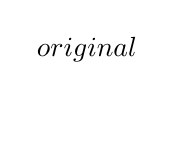
\begin{tikzpicture}        
		 \node [] (n0) at (0,0) {};
         \node [] (label) at (0,0.8) {$original$};
\end{tikzpicture}
&
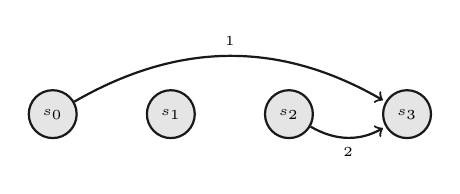
\begin{tikzpicture}[shorten >=1pt,->,scale=0.5]  
        \tikzstyle{sentence}=[circle,thick,draw=black!90,fill=black!10,minimum size=2mm]
		\tikzstyle{entity}=[circle,thick,draw=black!90,fill=black!10,minimum size=2mm]
        \tikzstyle{edge}=[draw=black!90, thick]

       \begin{scope}
       
         \node [sentence] (s0) at (0,0) {\tiny{$s_0$}};
         \node [sentence] (s1) at (3,0) {\tiny{$s_1$}};
         \node [sentence] (s2) at (6,0) {\tiny{$s_2$}}; 
         \node [sentence] (s3) at (9,0) {\tiny{$s_3$}}; 
 
 		\path[edge, bend left = 30] (s0) edge [above] node[font=\tiny]{$1$} (s3);
 		\path[edge, bend right = 30] (s2) edge [below] node[font=\tiny]{$2$} (s3);
           
        \end{scope}        
      \end{tikzpicture}

 &
 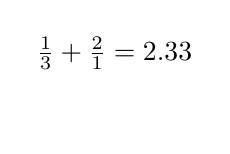
\begin{tikzpicture}        
		 \node [] (n0) at (0,0) {};
         \node [] (label) at (0,0.8) { $ \frac{1}{3} + \frac{2}{1}  = 2.33 $};
\end{tikzpicture}
&

\multirow{2}{*}{
\begin{tabular}{c}
$ 2.33 > 2 \Rightarrow $
\\
$correct$  
\end{tabular}
}
\\

&
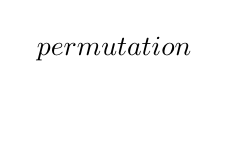
\begin{tikzpicture}        
		 \node [] (n0) at (0,0) {};
         \node [] (label) at (0,0.8) {$permutation$};
\end{tikzpicture}
&
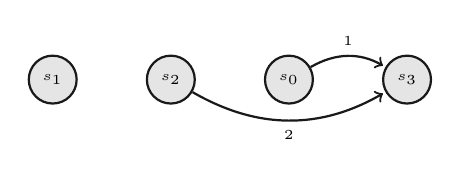
\begin{tikzpicture}[shorten >=1pt,->,scale=0.5]  
        \tikzstyle{sentence}=[circle,thick,draw=black!90,fill=black!10,minimum size=2mm]
		\tikzstyle{entity}=[circle,thick,draw=black!90,fill=black!10,minimum size=2mm]
        \tikzstyle{edge}=[draw=black!90, thick]

       \begin{scope}
       
         \node [sentence] (s1) at (0,0) {\tiny{$s_1$}};
         \node [sentence] (s2) at (3,0) {\tiny{$s_2$}};
         \node [sentence] (s0) at (6,0) {\tiny{$s_0$}}; 
         \node [sentence] (s3) at (9,0) {\tiny{$s_3$}}; 
 
 		\path[edge, bend left = 30] (s0) edge [above] node[font=\tiny]{$1$} (s3);
 		\path[edge, bend right = 30] (s2) edge [below] node[font=\tiny]{$2$} (s3);
           
        \end{scope}        
      \end{tikzpicture}

 &
 \begin{tikzpicture}        
		 \node [] (n0) at (0,0) {};
         \node [] (label) at (0,0.8) { $\frac{1}{1} + \frac{2}{2} =  2 $};
\end{tikzpicture}
&

\\ 
\hline
\\ 
\multirow{2}{*}{$P_{Acc}$ }
&

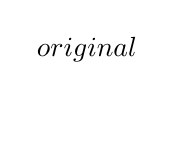
\begin{tikzpicture}        
		 \node [] (n0) at (0,0) {};
         \node [] (label) at (0,0.8) {$original$};
\end{tikzpicture}
&
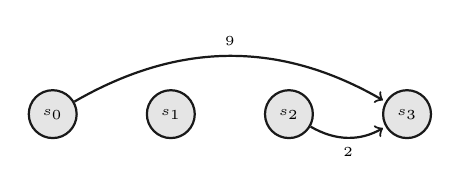
\begin{tikzpicture}[shorten >=1pt,->,scale=0.5]  
        \tikzstyle{sentence}=[circle,thick,draw=black!90,fill=black!10,minimum size=2mm]
		\tikzstyle{entity}=[circle,thick,draw=black!90,fill=black!10,minimum size=2mm]
        \tikzstyle{edge}=[draw=black!90, thick]

       \begin{scope}
       
         \node [sentence] (s0) at (0,0) {\tiny{$s_0$}};
         \node [sentence] (s1) at (3,0) {\tiny{$s_1$}};
         \node [sentence] (s2) at (6,0) {\tiny{$s_2$}}; 
         \node [sentence] (s3) at (9,0) {\tiny{$s_3$}}; 
 
 		\path[edge, bend left = 30] (s0) edge [above] node[font=\tiny]{$9$} (s3);
 		\path[edge, bend right = 30] (s2) edge [below] node[font=\tiny]{$2$} (s3);
           
        \end{scope}        
      \end{tikzpicture}

 &
 \begin{tikzpicture}        
		 \node [] (n0) at (0,0) {};
         \node [] (label) at (0,0.8) { $\frac{9}{3} + \frac{2}{1} = 5 $};
\end{tikzpicture}
&

\multirow{2}{*}{
\begin{tabular}{c}
$ 5 < 10 \Rightarrow $
\\
 $incorrect$
 \end{tabular}  
}
\\

&
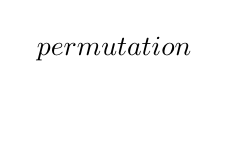
\begin{tikzpicture}        
		 \node [] (n0) at (0,0) {};
         \node [] (label) at (0,0.8) {$permutation$};
\end{tikzpicture}
&
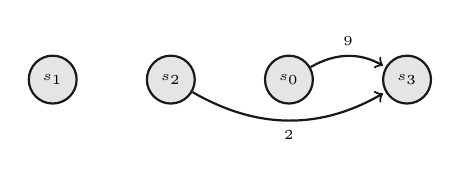
\begin{tikzpicture}[shorten >=1pt,->,scale=0.5]  
        \tikzstyle{sentence}=[circle,thick,draw=black!90,fill=black!10,minimum size=2mm]
		\tikzstyle{entity}=[circle,thick,draw=black!90,fill=black!10,minimum size=2mm]
        \tikzstyle{edge}=[draw=black!90, thick]

       \begin{scope}
       
         \node [sentence] (s1) at (0,0) {\tiny{$s_1$}};
         \node [sentence] (s2) at (3,0) {\tiny{$s_2$}};
         \node [sentence] (s0) at (6,0) {\tiny{$s_0$}}; 
         \node [sentence] (s3) at (9,0) {\tiny{$s_3$}}; 
 
 		\path[edge, bend left = 30] (s0) edge [above] node[font=\tiny]{$9$} (s3);
 		\path[edge, bend right = 30] (s2) edge [below] node[font=\tiny]{$2$} (s3);
           
        \end{scope}        
      \end{tikzpicture}

 &
 \begin{tikzpicture}        
		 \node [] (n0) at (0,0) {};
         \node [] (label) at (0,0.8) { $ \frac{9}{1} + \frac{2}{2} = 10 $};
\end{tikzpicture}
&
\\
\hline
\end{tabular}
\caption{An example of how syntactical roles vanish the effect of the distance information.}
\label{table:pacc_vanishing_problem}
\end{figure}

This example shows $P_W$ and $P_{Acc}$ of the same document. 
It is clear from the $P_W$ presentation of the original order of the document that in the entity graph representation of the document, sentence node $s_3$ shares respectively one and two entity nodes with sentence nodes $s_0$ and $s_2$. 
The weights of edges in $P_{Acc}$ representation of the original order depict that grammatical transition of the common entity between $s_0$ and $s_3$ is $S\ S$, because the weight of the edge between these two nodes is $9$ and $S$ is mapped to $3$. 
With the same reasoning, we can induce that the grammatical transitions of two common entities between $s_2$ and $s_3$ are $X\ X$. 
In Table \ref{table:pacc_vanishing_problem}, we compare the original outdegree of projection graphs that represent the original order of sentences and one of its permutations in that $s_0$ is removed from the original order and reinserted in the third position between $s_2$ and $s_3$. 
This example shows how the way of computing the weights of projection graphs affect the performance of the graph-based coherence model for the insertion task. 
As we discussed before an important factor in sentence ordering tasks is distance and 
 accumulating the associated numbers to the grammatical roles of entities discards the effect of distance. 
However, the difference between the accuracy of the $P_{Acc}$ and $P_{W}$ is not statistically significant and this difference can be ignored. 

Interestingly, $P_{Acc}$ obtains a better accuracy than $P_W$ in the discrimination task. 
This can be explained in this way that in the insertion task the weights of edges that are only connected to the removed/reinserted sentence node change and the weight of all other edges do not change. 
Contrary, in the discrimination task the position of most sentences are changed. 
Weights of most edges get updated and it is less likely that all weights vanish.
Therefore, it is more likely in the discrimination task that new weights help to make more correct decisions. 


The second column of Table \ref{table:insertion_result} shows the insertion score of different models on the insertion task. 
The insertion score -- the higher, the better -- measures how near the proposed position for a removed sentence is to its original position. 
We can see that the insertion scores obtained by our normalization model is higher than the one provided with the entity grid model.
However, the entity grid model (E\&S) reaches a higher insertion score. 
This means that, if it makes more mistakes than our system, the position chosen by the entity grid model is usually closer to the correct position. 


\subsection{Summary Coherence Ranking}
%
Sentence ordering task do not measure all aspects of coherence. 
Admittedly, the synthetic data used in the ordering tasks partially approximate coherence violations that human readers encounter in machine generated texts. 
The summary coherence ranking task is based on this intuition that a coherence model that exhibits a high agreement with human judges accurately captures the coherence properties of the machine generated texts. 
In this task, we test the ability of our coherence models to assess coherence by comparing rankings induced by a model against rankings elicited by human judges. 
Moreover, this task more close to real application of coherence in automatic text summarization.

We use the dataset proposed and used by \newcite{barzilay08} to evaluate their  coherence model (i.e., the entity grid model).  
The dataset contains $80$ pairs of summaries extracted from Document Understanding Corpus (DUC) $2003$. 
The corpus used in DUC 2003 includes multi-document summaries generated by human writers and by automatic summarization systems. 
In order to learn a ranking, we require a set of summaries, each of which has been rated in terms of coherence. 
This ratings are not provided by DUC summary evaluators. 
In DUC $2003$, the quality of system generated summaries was assessed with respect to several factors ranging from grammar, to content selection, fluency, and readability. 
Coherence was indirectly evaluated by noting the number of sentences indicating an awkward time sequence, suggesting a difficult to interpret relationship between sentences, or being semantically incongruent with their other sentences. 
\newcite{barzilay08} obtained judgments for automatically generated summaries from human subjects\footnote{\url{http://homepages.inf.ed.ac.uk/mlap/coherence/}}.
They randomly selected $16$ input documents and five systems that had produced summaries for these documents, plus the reference summaries written by humans. 
Coherence ratings were collected during an elicitation study by $177$ unpaid volunteers, all native English speakers. 
Participants first saw a set of instructions that explained the task, and defined the notion of coherence using multiple examples. 
The summaries were randomized in lists following a Latin square design ensuring that no two summaries in a given list were generated from the same document cluster. 
Participants were asked to use a seven-point-scale to rate how coherent the summaries were without having seen the source texts. 
The ratings (approximately $23$ per summary) given by our subjects were averaged to provide a rating between $1$ and $7$ for each summary. 
In order to to validate the quality of the annotations of how well humans agree in their coherence assessment, several tests have been done such as leave-one-out re-sampling, by correlating the data obtained from each participant with the mean coherence ratings obtained from all other participants. 
The inter-subject agreement was $r = 0.768$ ($p < 0.01$). 
In another annotation qualification test, they examined the effect of different types of summaries (human- vs. machine-generated.) concluding that human summaries are perceived as significantly more coherent than system-generated ones. 
The set of training materials contained $6 × 16$ summaries (average length $4.8$), yielding $c(6,2) × 16 = 240$ pairwise rankings. 
Because human summaries often have identical (high) scores, pairs of such summaries from the training set have been eliminated. 
Consequently, the resulting training corpus consisted of $144$ summaries. 
In a similar fashion, $80$ pairwise rankings for the test set have been obtained. 
Human coherence scores are associated with each pair of summarized documents \cite{barzilay08} Each of pair of the test set is being composed by two summaries of a same document where the score of one of the summaries is significantly higher than the score of the second one. 
Even though all summaries are of approximately the same length ($114.2$ words on average), their sentence length can vary considerably. 
Indeed, more coherent summaries tend to have more sentences and contain less entities


Considering this setting, Summary coherence rating can be also formulated as a ranking learning task.
Given a pair of summaries, one more coherent than the other, the objective of the task is to order the two summaries according to local coherence.

For evaluation purposes, similar to the discrimination  in the sentence ordering task, we use  accuracy and F-measure where the former corresponds to the number of correct ranking divided by the number of comparisons, and the latter the average of recall and precision measures.
As before, significance is tested with the Student’s t-test accounting for the Bonferroni correction.


\begin{table}[!t]
\centering
\begin{small}
\begin{tabular}{l|cc@{}l}
 & Acc. & F  &\\\hline
 B\&L & $0.833$ &  &\\\hline

 & \multicolumn{3}{|c}{Entity graph, G\&S} \\\hline 
$P_U$ & $0.800$ & $0.815$ &  \\
$P_W$ & $0.613$ & $0.613$&* \\
$P_{Acc}$ & $0.700$ & $0.704$& \\  
$P_U$, \textit{Dist} & $0.650$ & $0.658$ \\
$P_W$, \textit{Dist} & $0.525$ & $0.525$  \\
$P_{Acc}$, \textit{Dist} & $0.700$ & $0.700$  \\
\hline 

 & \multicolumn{3}{|c}{Normalized entity graph} \\\hline 
$P_U$ & $\textbf{0.800}$ & $\textbf{0.815}$&  \\
$P_W$ & $0.775$ & $0.775$& \\
$P_{Acc}$ & $0.788$ & $0.788$& \\  
$P_U$, \textit{Dist} & $0.650$ & $0.658$ \\
$P_W$, \textit{Dist} & $0.738$ & $0.738$  \\
$P_{Acc}$, \textit{Dist} & $0.750$ & $0.750$  \\
\end{tabular}
\end{small}
\caption{Summary Coherence Rating, B\&L and entity
  graph vs.\ normalized entity graph}
 \label{table:summary_coherence_ranking}
\end{table}
%%%%%%%%%%

Table \ref{table:summary_coherence_ranking} displays reported results of $B\&L$ and reproduced results of the entity graph and our normalized entity graph. 
Unlike the sentence ordering task, accounting for the distance information between two sentence nodes (\textit{Dist}) tends to decrease the performance of graph models. 
This difference is explained by the fact that a human summary, which is usually considered more coherent by humans judges, is inclined to contain more (and shorter) sentences than a summary generated by machines. 
As adding distance information diminishes the value of our local coherence score (i.e. outdegree), distinguishing between the coherence and incoherent summaries becomes more difficult. 
Therefore, both graph-based models obtain better results without incorporating the distance information. 


Moreover, in contrast to the sentence ordering experiment, when we employ the number of entities ``shared” by two sentences as weights of projection graphs ($P_W$), models obtain lower values of accuracy and F-measure, than $P_U$. 
This behavior could be because the number of sentences contained in the less coherent summaries. 
Summaries generated by machines contain a smaller number of sentences where each sentence contains more entities on average. 
This means that, in these summaries, two sentences are more likely to share a larger number of entities and therefore have a
higher local coherence score when the $P_W$ projection graph is used.  
The $P_{Acc}$ in the entity graph models obtains slightly better accuracy and F-measure than $P_W$. 


Normalizing significantly improves the results of $P_W$  and $P_{Acc}$. 
With the same reason to the entity graph model, distance information degrades the results for the normalization graph too. 
$P_U$ is still slightly better than both $P_W$ and $P_{Acc}$, but in contrast to the entity graph, this difference is not statistically significant showing an advantage of our normalization method. 
In the entity graph model, three projection graphs are proposed and as Table \ref{table:summary_coherence_ranking} shows their results are statistically different. 
Our normalization method makes the difference between the results negligible. 
So in production, there would be no difference between different projection graphs if the normalization method is used. 



\subsection{Readability Assessment}
%
Readability describes how easily a document can be read and understood. 
Some research papers \cite{} estimate the difficulty of a document by means of the time with that a reader can process and understand the document. 
Indeed, the difficulty of a document for its readers is beyond the surface aspects of the document such as employed vocabularies, the length of sentences, and etc. 
Discourse level factors of a document (e.g. coherence) plays a critical role in overall understanding of the document. 
Sentences of more coherent documents are supposed to be connected so that sentences become less ambiguous and information flow smoothly through the document. 

The task of readability assessment aims to distinguish texts which are difficult to read from texts which are easier to read. 
Following \cite{guinaudeau13}, we treat the readability assessment task as a ranking task.
Given a pair of document which one is easier to read. 

We use the readability dataset collected\footnote{\url{http://homepages.inf.ed.ac.uk/ mlap/coherence/.}} by \newcite{barzilay03b}, and used by \newcite{barzilay08,guinaudeau13}, from the Encyclopedia Britannica and Britannica Elementary. 
The former contain the original and full articles and the latter version is targeted at children. 
The dataset contains $107$ articles from the full version of the Encyclopedia Britannica and their corresponding simplified articles from Britannica Elementary ($107 + 107 = 214$ articles in total).
Although these texts are not explicitly annotated with readability levels, they still represent two broad readability categories, namely, difficult and easy. 
The collected articles of Encyclopedia Britannica are longer than their corresponding articles of Britannica Elementary in terms of number of sentences ($83.1$ sentences vs $36.6$ on average). 


In order to estimate the complexity of a text, the graph-based coherence models compute the local coherence score for each text in the two categories.  
Texts associated with the higher score is considered to be the more readable as it is more coherent, needing less interpretation from the reader than a text associated with a lower local coherence score. 


As before, we evaluate coherence models using accuracy and F-measure metrics. 
The accuracy measures how often a coherence model correctly distinguishes the version of an article from Encyclopedia Britannica more difficult than its version from Britannica Elementary. 
F-measure is also computed based on the precision and recall as explained in previous experiments. 

We compare graph-based coherence models (i.e., the entity graph model and the normalized entity graph model) with the entity grid model (B\&L) as a coherence model, (S\&O) as a readability assessment model, and (B\&L $+$ S\&O) that is taken as an enriched readability assessment model with proposed coherence features in B\&L. 


Table \ref{table:bri_ele} summaries the results of these models. 

\begin{table}[!t]
\centering
\begin{small}
\begin{tabular}{l|cc@{}l} 
  & Acc. & F  &\\\hline
  S\&O & $0.786$ & &\\
  B\&L & $0.509$ &  &\\
  B\&L $+$ S\&O & $0.888$ & &\\\hline

  & \multicolumn{3}{|c}{Entity graph, G\&S} \\\hline 

  $P_U$, \textit{Dist} & $0.589$ & $0.589$ &**  \\
  $P_W$, \textit{Dist} &  $0.570$ & $0.570$ &**  \\
  $P_{Acc}$, \textit{Dist} & $0.766$ & $0.766$ &** \\\hline 
	& \multicolumn{3}{|c}{Normalized entity graph} \\\hline 

  $P_U$, \textit{Dist} & $0.589$ & $0.589$&**  \\

  $P_W$, \textit{Dist} & $\textbf{0.897}$ & $\textbf{0.897}$&  \\
  $P_{Acc}$, \textit{Dist} & $0.850$ & $0.850$&

\end{tabular}
\end{small}
\caption{Readability assessment, baselines and entity graph vs.\
  normalized entity graph}
\label{table:bri_ele}
\end{table}


Distance information always improves the results. 
For this task, syntactic information plays a dominant role ($P_Acc$) in the entity graph model.
A statistically significant ($p < 0.01$)  improvement is provided by including syntactic information in comparison with $P_U$, \textit{Dist} and $P_W$, \textit{Dist} in the entity graph model.   
$P_{Acc}$, \textit{Dist} considers a higher weight for subject entities that are more frequent in the Britannica Elementary documents which are composed by simpler and shorter sentences.


Table \ref{table:bri_el} also shows that when the number of entities ``shared” by two sentences is accounted for ($P_W$), the results are lower. 
Indeed, Encyclopedia Britannica documents are composed by longer sentences, that contain a higher number of entities. 
This increases the local coherence value of difficult documents more than the value of “easy to read” documents, that contain less entities. 

Interestingly, the entity graph model (B\&L) that captures exclusively local coherence is almost on par with the accuracy reported by S\&O \cite{schwarm05} system, which relies on a wide range of lexical, syntactic and semantic features. 
Only when \newcite{barzilay08} combine the entity grid with S\&O features they reach performance considerably better than the best performance of the entity graph model. 

The best performing system on the experimented readability assessment task is the normalized entity graph model. 
The normalized entity graph ($P_W, Dist$) does not only outperform the entity graph (significantly) and B\&L, but also S\&O and the combination B\&L $+$ S\&O. 
The normalized entity graph outperforms the entity graph because it incorporates the effect of entities not shared between sentences when it computes the weight of projection graphs. 
Sentences in the \emph{Britannica Elementary} are simpler and shorter than in the \emph{Encyclopedia Britannica}.
Hence, \emph{Britannica Elementary}\ receives a higher cohesion score than \emph{Encyclopedia Britannica}\ in our
model. 
Adding grammatical information, does not help, because of the influence of the number of entities (shared and not shared) outweighs the influence of syntactic roles. 

Similar to the results of the normalized entity graph on summary coherence ranking task, our normalization method not only improve the performance of the entity graph model, it pushes the results of different projection graphs closer to each other. 

 
In another experiment, following \cite{guinaudeau13} we use a third readability category, the Britannica Student (Stud.), that contains articles targeted for youths (from $11$ to $14$ years old). 
These documents, which are quite similar to the Encyclopedia Britannica ones, are composed by an average of $44.1$ sentences. 
Only $99$ articles out of the $107$ original ones are used in this experiment were available in Britannica Student, so sub corpora of the twp categories were used for the comparison with the Britannica Student articles

\begin{table}[!t] 
 \centering
 \begin{tabular}{l|cc|cc} 
  \multicolumn{5}{c}{Standard graph-based model}\\\hline
  & \multicolumn{2}{|c}{\textit{Brit.\ vs.\ Stud.}} &
	\multicolumn{2}{|c}{\textit{Stud.\ vs.\ Elem.}}\\\hline 
  & Acc. & F & Acc. & F\\\hline
   $P_U$ & $0.444$ & $0.444$ & $0.667$ & $0.667$\\
   $P_W$ & $0.434$ & $0.434$ & $0.636$ & $0.636$\\ 
   $P_{Acc}$ & $0.465$ & $0.465$ & $0.707$ & $0.707$\\
   $P_U$, \textit{Dist} & $0.475$ & $0.475$ & $0.646$ & $0.646$\\
   $P_W$, \textit{Dist} & $0.485$ & $0.485$ & $0.616$ & $0.616$\\
   $P_{Acc}$, \textit{Dist} & $0.556$ & $0.556$ & $0.657$ & $0.657$\\\hline 
  
    \multicolumn{5}{c}{Normalized graph-based model}\\\hline
   $P_U$ & $0.444$ & $0.444$ & $0.667$ & $0.667$\\
   $P_W$ & $0.515$ & $0.515$ & $0.778$ & $0.778$\\ 
   $P_{Acc}$ & $0.515$ & $0.515$ & $0.768$ & $0.768$\\
   $P_U$, \textit{Dist} & $0.475$ & $0.475$ & $0.646$ & $0.646$\\
   $P_W$, \textit{Dist} & $\textbf{0.657}$ & $\textbf{0.657}$ & $0.758$ & $0.758$\\
   $P_{Acc}$, \textit{Dist} & $0.646$ & $0.646$ & $\textbf{0.788}$ & $\textbf{0.788}$\\
 \end{tabular}
 \caption{Readability, comparison between \emph{Encyclopedia Britannica}, \emph{Britannica Elementary} and \emph{Britannica Student}}
 \label{t:exp3:stu}
 \end{table}

\textit{Britannica Student} is another version of \textit{Encyclopedia Britannica} which are provided for youths \cite{guinaudeau13}. 
The content of their articles are similar.

Table \ref{t:exp3:stu} shows the results obtained for the comparisons between the two first categories (i.e., Encyclopedia Britannica (\textit{Brit.}) and Britannica Elementary (\textit{Elem.})) and the Britannica Student (\textit{Stud.}) articles. 
When articles from Britannica Student are compared to articles extracted from Encyclopedia Britannica, Table \ref{t:exp3:stu} shows that the different parameters have the same influence as for comparing between Encyclopedia Britannica and Britannica
Elementary: statistically significant improvement with syntactic information, higher values when distance is taken into account, etc.
However, it can also be seen that accuracy and F-measure are lower for comparing these two corpora. 
This is probably due to the stylistic difference between these two kinds of categories, which is less significant than the difference between articles from Encyclopedia Britannica and Britannica Elementary.

These two additional experiments show that the entity graph model is also style dependent. 
It obtains better results when it has to distinguish between Encyclopedia Britannica and Britannica Elementary or Britannica Student and Britannica Elementary articles which present a more important difference from
a stylistic point of view than articles from Encyclopedia Britannica and Britannica Elementary.

When we compare the results of the normalized entity graph model with the entity graph model, it significantly outperforms the entity graph model on both comparisons. 
Interestingly, the normalized version of $P_{Acc}$, \textit{Dist.} obtains the highest performance in distinguishing articles of \textit{Stud.} from \textit{Ele.}. 
This can be interpreted in this way that due to the almost similar average sentence length of articles in \textit{Stud.} and \text{Ele.} datasets, the impact of syntactical information is more visible. 

\textbf{
The average number of sentences in articles of \textit{Stud.} is closer to the average number of sentences in articles of \textit{Ele.} than those of articles in \textit{Bri.} 
( $44.1$ vs $36.6$ vs $83.1$ ). 
This means the the average sentence length of \textit{Stud.} and \textit{Ele.} is also almost similar. 
In other words, the number entities mentioned in each sentence is on average similar between these two dataset. 
So we expect that the distributions of entities shared or not shared by sentences are kind of similar and syntactical information or the way that entities are referred by sentences is more discriminative information. 
}


As previously, coreference resolution tends to lower the results, therefore only values obtained without coreference resolution are reported in the table.

\section{Related Work}
%
In this section, we refer to related research to each part of this chapter. 

Different extensions of the entity grid model are introduced in Section \ref{}. 
The entity graph model also has been extended by from different perspectives. 
\cite{petersen15} use several graph topology metrics to approximate different aspects of the discourse flow that can indicate coherence, such as the average clustering or betweenness of discourse entities in text. 
They investigate if graph properties, such as the clustering coefficient, or iterative graph ranking algorithms, such as PageRank,  can approximate document coherence. 
They conclude that the topological metrics that their employed to model the topology of graphs work on par with the average outdegree employed by  entity graph. 

\cite{dias15}  fill the grid in the entity grid with the occurrence of discursive information
(RST and/or CST \cite{?}(Castro Jorge et al. 2014)) such that an entry is one where an entity is part of a sentence that participate in a discursive relation.
Then define the bipartite graph as its original version ans use outdegree to measure coherence of texts. 
Their model outperforms the entity graph model for sentence ordering task on summaries produced by a multi-document summarizer. 
This may be justified by the availability of more CST relations than RST relations in multi-document summaries.
They argue that although the new information improve the results, obtaining discursive information is expensive. 

\cite{lioma16} eliminate the need for the projection graph with this intuition that projection incur significant loss of information present in bipartite graph.  
They present three new graph metrics that compute text coherence on the original bipartite graph. 
These metrics are obtained by different ways of normalizing the weights of the entity graph representation. 
That is different with our approach that normalize the weights of the projection graphs and uses outdegree as the final coherence score. 

% Centering has been applied directly in models of coherence (Karamanis et al., 2004; Karamanis et al., 2009); other models use the basic Centering principles as soft constraints or features in a probabilistic framework such as the Entity Grid (Lapata and Barzilay, 2005), which we discuss them in more details in following sections. 
% Givon’s (1987) and Hoey’s (1991) accounts of discourse continuity complement local measurements by considering global characteristics of entity distribution, such as the life time of an entity in discourse and the referential distance between subsequent mentions. 
% A great deal of research has been devoted to this issue, primarily in Centering Theory (Miltsakaki and Kukich 2000; Hasler 2004; Karamanis et al. 2004).
 
%e.g. work on word sense
%disambiguation by Navigli and Lapata (2010); for
%an overview over graph-based methods in NLP
%see Mihalcea and Radev (2011)) 

%%%%%%%%%%%%%%%%%%%%%%%%%%%%%%%%%%%%%%%%%%5
\section{Conclusions}
%
In all experiments that have been done in this chapter, the normalized entity graph outperformed the entity graph model. 
An important observation was that different weighted projection graphs obtain almost similar performance when the normalized entity graph is applied. 
The difference between their results is not statistically significant showing that we may use a unique projection graph. 
Since the normalized $P_w$ works the best for most experiments in this chapter, it seems that this projection graph can be used instead of other projection graphs as a default setting. 
The results of our experiments on the readability assessment task indicate that when the datasets on that we are experimenting have a similar style (e.g. similar sentence length), the projection graph that incorporates the syntactical information works better than $P_W$, not significantly though. 

Experiments related to sentence ordering (i.e., discrimination, and insertion) show that  incorporating the distance between sentences with projection graphs obtains very high performance while coherence is beyond the distance between sentences. 
High performance of graph-based models on sentence ordering tasks, indeed, indicates that the sentence ordering task is too artificial for evaluating coherence models. 
In following chapters, we evaluate our coherence models on real NLP applications in that coherence plays an important role. 

Overall, we conclude in this way that the entity graph representation is a  more suitable framework for coherence modeling.  
Since it defines the distribution of entities among sentences via a graph, it does not face with the sparsity issue $- -$ of the entity grid model that uses a matrix. 
Moreover, this representation is designed linguistically and is not data driven. 
In terms of modeling, being independent from data is a pros for the entity graph model. 
However, there is always some information in data that machine learning models can learn them automatically. 
For example, what factors of the entity graph representation of texts are more important for each task. 
The entity graph model employs the average outdegree of sentence nodes in the projection graphs as the only factor to encode the connectivity of sentences nodes and consequently the connectivity of their corresponding sentences. 
So far, we realized that the graph representation is more informative than grid for coherence modeling.
In next chapter, we focus on the average outdegree and check how informative it is for coherence measurement. 

































